%-----------------------------------------------------------------------------%
\chapter{\babEmpat}
%-----------------------------------------------------------------------------%
Bab ini menunjukkan hasil dari studi kinerja LDPC \textit{codes} DVB-T2 pada kanal AWGN dan \textit{channel model} DVB-T2 Indonesia. Bab ini juga menganalisis \textit{degree distribution} LDPC \textit{codes} DVB-T2 yang diusulkan dengan menggunakan EXIT \textit{chart} beserta validasinya menggunakan parameter praktis BER dan jumlah \textit{girth}.



\section{Analisis EXIT \textit{Chart} LDPC \textit{Codes} DVB-T2 pada Kanal AWGN}

Tugas Akhir ini menganalisis kinerja LDPC \textit{codes} DVB-T2 menggunakan EXIT \textit{chart} berdasarkan \textit{degree distribution} setiap \textit{code rate} dari LDPC \textit{codes} yang terbentuk. EXIT \textit{chart} mengeplot \textit{mutual information} di titik $V$ dan $C$ yang ditunjukkan pada proses \textit{iterative decoding} LDPC \textit{codes}. Secara praktis informasi ini diwakili oleh LLR, \textit{iterative decoding} pada LDPC \textit{codes} menukar LLR antara VND dan CND melalui \textit{edge} yang menghubungkan keduanya. \textit{Mutual information} yang terlibat adalah $ I_ {A, C} , I_ {E, C} , I_ {A, V} , I_ {E, V} $ seperti pada Gambar \ref{gambar: exit2} dan \ref{fig:exit49} mengekspresikan \textit{mutual information} yang masuk ke CND, \textit{mutual information} yang keluar dari CND, \textit{mutual information} yang masuk ke VND, dan \textit{mutual information} yang keluar dari VND pada iterasi LDPC \textit{codes}. Gambar \ref{gambar: exit2} menunjukkan EXIT \textit{chart} untuk \textit{code rate} $R_e=\frac{4}{9}$ untuk semua LDPC \textit{codes} DVB-T2 yang diusulkan pada SNR $\gamma=2.25$~dB dan menunjukkan EXIT \textit{chart} untuk \textit{code rate} $R_e=\frac{3}{5}$ untuk semua LDPC \textit{codes} DVB-T2 yang diusulkan pada SNR $\gamma=3.75$~dB. Gambar \ref{fig:exit49} menunjukkan EXIT \textit{chart} untuk \textit{code rate} $R_e=\frac{2}{3}$ untuk semua LDPC \textit{codes} DVB-T2 yang diusulkan pada SNR $\gamma=4$~dB.



Tugas Akhir ini mengalisis EXIT \textit{chart} pada setiap LDPC \textit{codes} DVB-T2 yang diusulkan pada kanal AWGN dalam dua dimensi (2D). Untuk mempermudah analisis, Tugas Akhir ini mengukur \textit{mutual information} menggunakan fungsi $J$ dan $J^{-1}$. Hubungan antara varians dan \textit{mutual information} adalah \cite{exit1}

\begin{eqnarray}
\sigma &=& J^{-1}({I_{A}}),\\
I&=&J(\sigma)
\end{eqnarray}
\begin{figure}
	\centering
	%	\hspace{-0.2 in}
	\begin{minipage}{1\linewidth}
		\hspace{0.75 cm}
		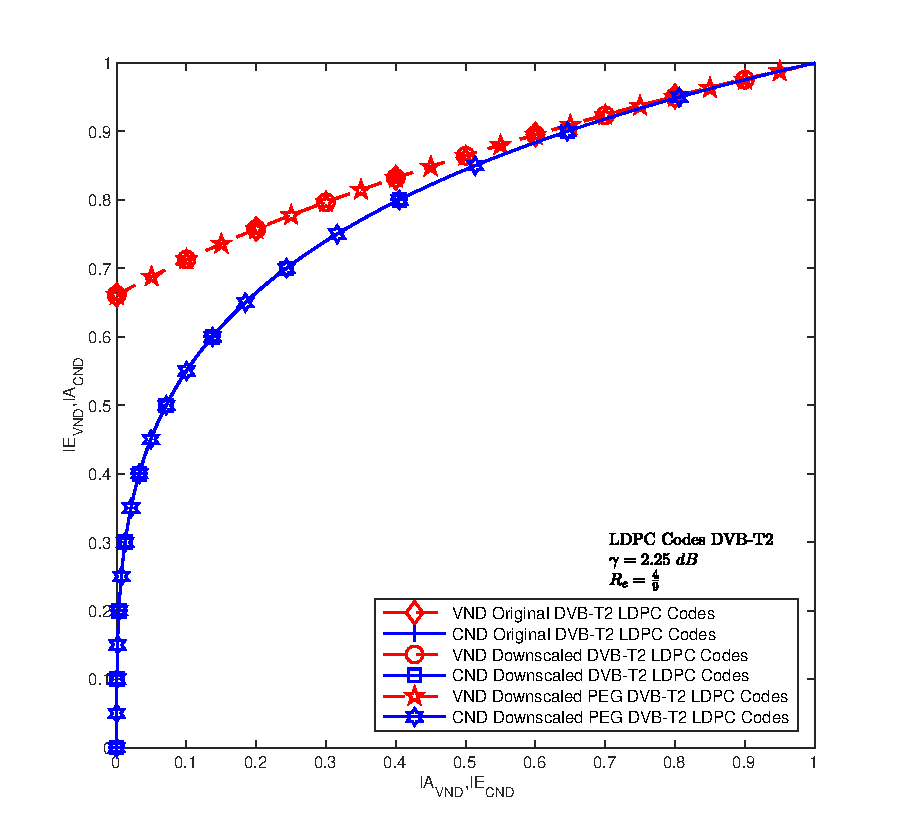
\includegraphics[width=0.85\textwidth]{pics/exit/12/12semua=snr2,25Ich=0,6613.pdf}
		\vspace{-1cm}
		
		\center  (a)
	\end{minipage}
	\hfill
	\begin{minipage}{1\linewidth}
		\hspace{0.75 cm}
		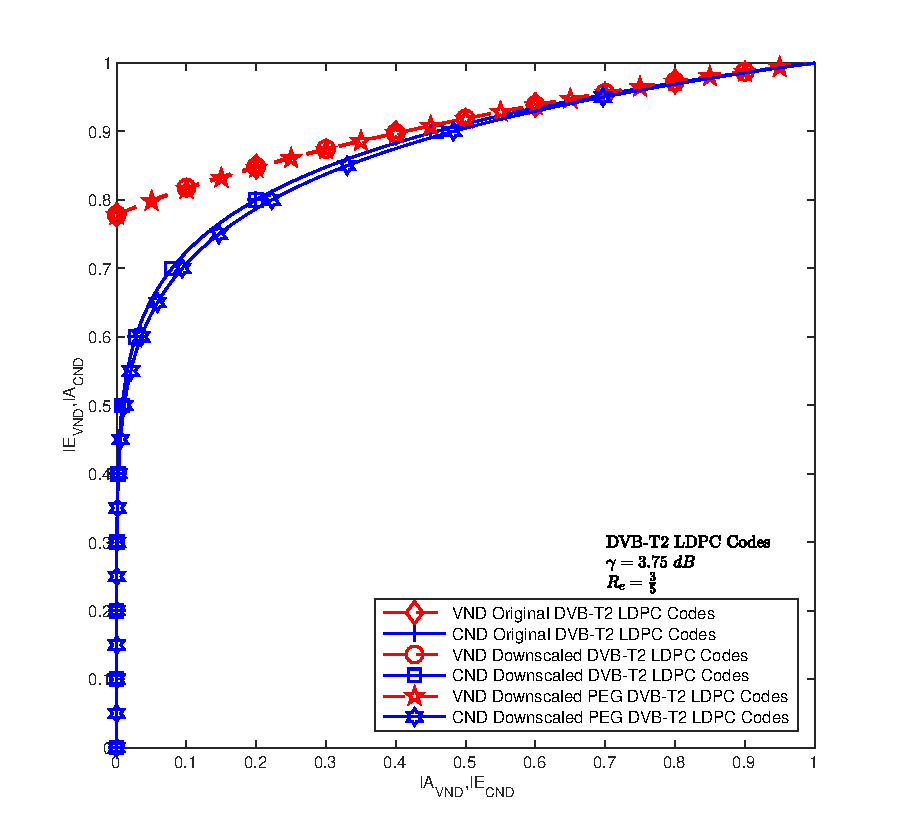
\includegraphics[width=0.85\textwidth]{pics/exit/35/35semua=snr3,75Ich=0,7786.pdf}
		\vspace{-1cm}
		\center (b)
	\end{minipage}
	%	\begin{minipage}{.5\linewidth}
	%		\hspace{-0.4 cm}
	%		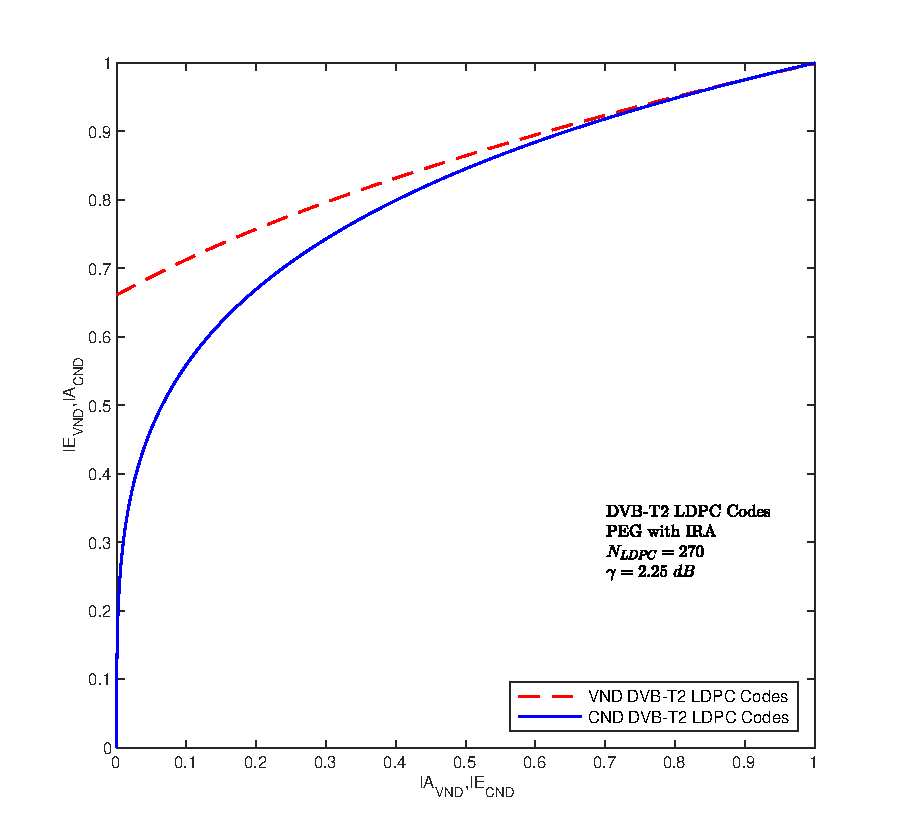
\includegraphics[width=3in]{pics/exit/12/12peg=snr2,25Ich=0,6613.pdf}
	%		\vspace{-1cm}
	%		\center (c)
	%	\end{minipage}
	\caption {Analisis EXIT \textit{chart} LDPC \textit{codes} DVB-T2 dengan (a) $R_e=\frac{4}{9}$ dan (b) $R_e=\frac{3}{5}$, masing-masing, pada SNR $\gamma=2,5~dB$ dan $\gamma=3,75~dB$.}
	\label{gambar: exit2}
\end{figure}\begin{figure}[t!]
\centering
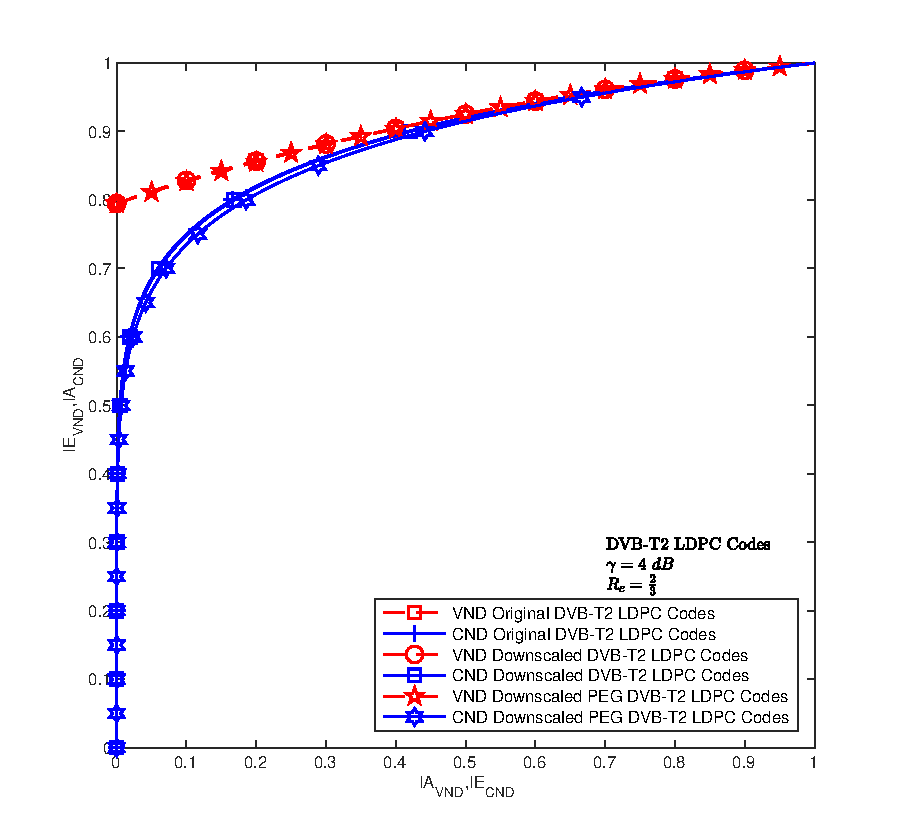
\includegraphics[width=1\textwidth]
{pics/exit/23/23semua=snr4Ich=0,795.pdf}
\caption{Analisis EXIT \textit{chart} LDPC \textit{codes} DVB-T2 dengan $R_e=\frac{2}{3}$ pada SNR $\gamma=4~dB$.}
\label{fig:exit49}
\end{figure} 
\noindent dengan $\sigma^2 = \frac{4}{\sigma_n^2}$,  $\sigma_n^2$ adalah \textit{noise variance}.  EXIT \textit{chart} dalam Tugas Akhir ini mengeplot berdasarkan \textit{mutual information}
\begin{equation}
I_{E,V}\! =\! \sum_i \mathcal{F}_i^\Lambda { J\left( \sqrt{(d_{V_i}\!-\!1)[J^{-1}(I_{A,V})]^2\!+\! [J^{-1}(I_{A_{CH}})]^2}\right)}
\label{eq:I_E_V_int}
\end{equation} 
dengan $\mathcal{F}_i^\Lambda$ adalah pecahan ke-$i$ dari $\Lambda_{LDPC}(x)$ dan 
\begin{equation}
I_{E,C} = 1-\sum_i \mathcal{F}_i^\Omega J\left( \sqrt{(d_{C_i}-1)[J^{-1}(1-I_{A,C})]^2}\right)
\end{equation}
dengan $\mathcal{F}_i^\Omega$ adalah pecahan ke-$i$ pada $\Omega_{LDPC}(x)$. Parameter $I_{A_{CH}}$ adalah \textit{mutual information} yang berasal dari \textit{channel}.


Gambar \ref{fig:exit3} menunjukkan EXIT \textit{chart} untuk \textit{code rate} $R_e=\frac{11}{15}$ untuk semua LDPC \textit{codes} DVB-T2 yang diusulkan pada SNR $\gamma=4.25$~dB. Gambar \ref{gambar: exit737} menunjukkan EXIT \textit{chart} untuk \textit{code rate} $R_e=\frac{11}{15}$ untuk semua LDPC \textit{codes} DVB-T2 yang diusulkan pada SNR $\gamma=4.5$~dB dan menunjukkan EXIT \textit{chart} untuk \textit{code rate} $R_e=\frac{37}{45}$ untuk semua LDPC \textit{codes} DVB-T2 yang diusulkan pada SNR $\gamma=5.25$~dB.

EXIT \textit{chart} menunjukkan celah kecil yang membuktikan distribusi derajat yang baik, celah terbuka pada EXIT \textit{chart} bermanfaat untuk memulai decoding di awal kurva. Evaluasi EXIT \textit{chart} pada Tugas Akhir ini menunjukkan semakin besar \textit{code rate}, maka nilai SNR untuk mencapai kurva EXIT yang baik semakin besar. Setiap kurva EXIT \textit{chart} menunjukkan bahwa original LDPC \textit{codes} memiliki EXIT \textit{chart} yang sedikit lebih baik daripada LDPC \textit{codes} DVB-T2 yang diusulkan, sehingga membuktikan bahwa \textit{downscaled} LDPC \textit{codes} dapat memiliki kinerja yang tidak jauh beda daripada original LDPC \textit{codes}.
\begin{figure}[b!]
	\centering
	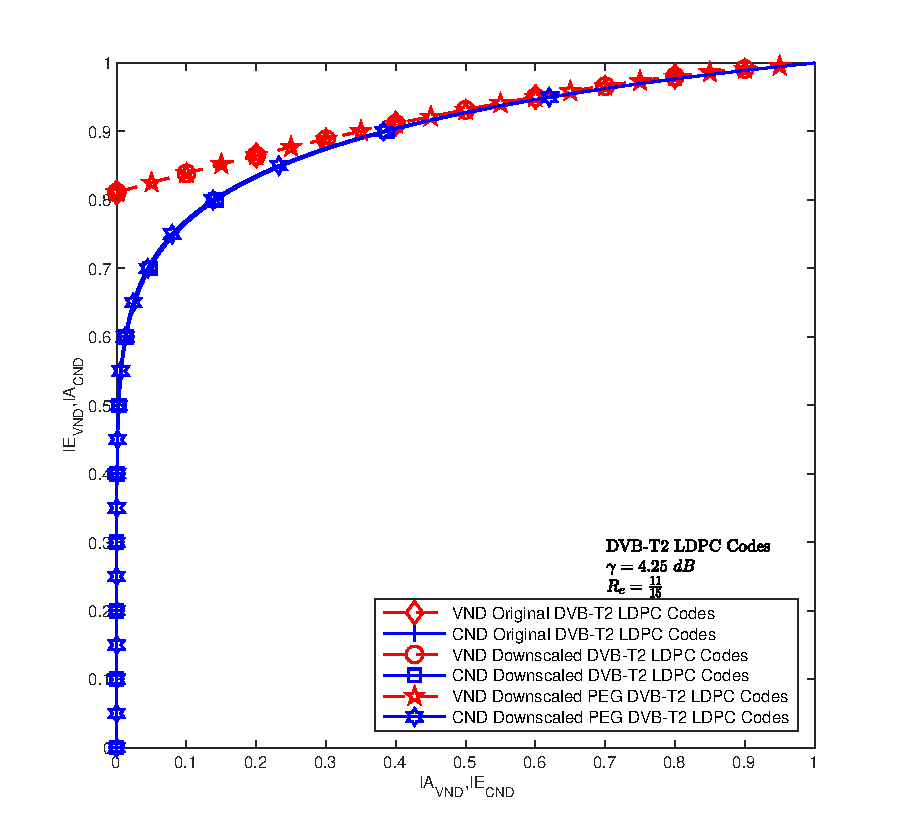
\includegraphics[width=1\textwidth]
	{pics/exit/34/34semua=snr4,25Ich=0,8113.pdf}
	\caption{Analisis EXIT \textit{chart} LDPC \textit{codes} DVB-T2 dengan $R_e=\frac{11}{15}$ pada SNR $\gamma=4,25~dB$.}
	\label{fig:exit3}
\end{figure}
\begin{figure}[H]
	\centering
	%	\hspace{-0.2 in}
	\begin{minipage}{1\linewidth}
		\hspace{0.75 cm}
		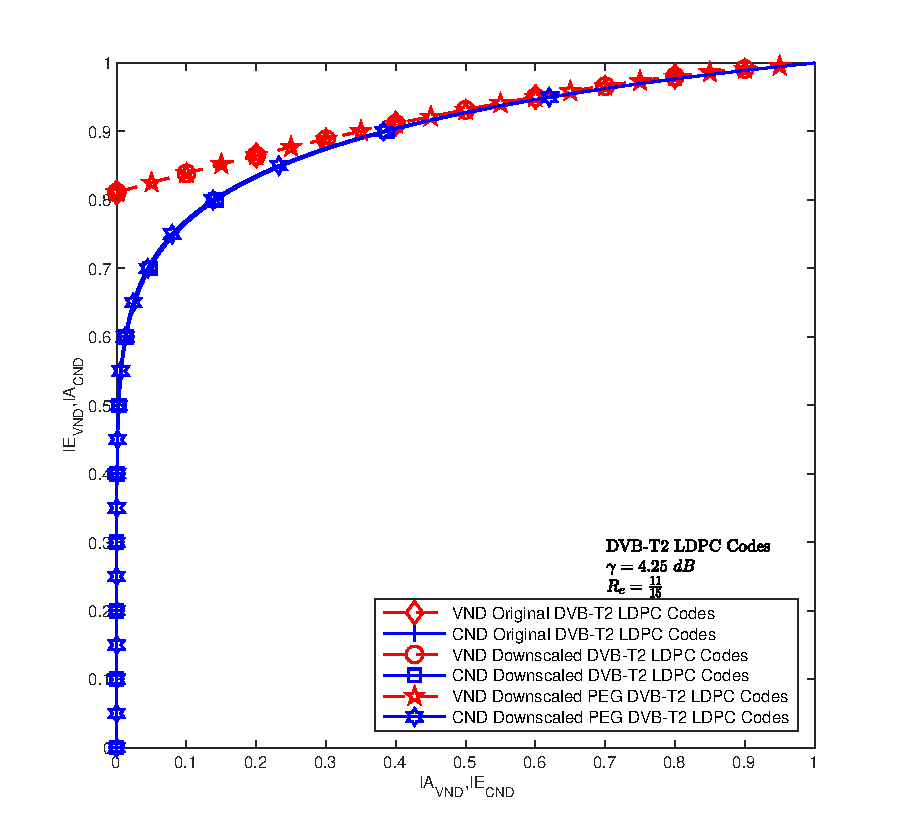
\includegraphics[width=0.85\textwidth]{pics/exit/34/34semua=snr4,25Ich=0,8113.pdf}
		\vspace{-1cm}
		
		\center  (a)
	\end{minipage}
	\hfill
	\begin{minipage}{1\linewidth}
		\hspace{0.75 cm}
		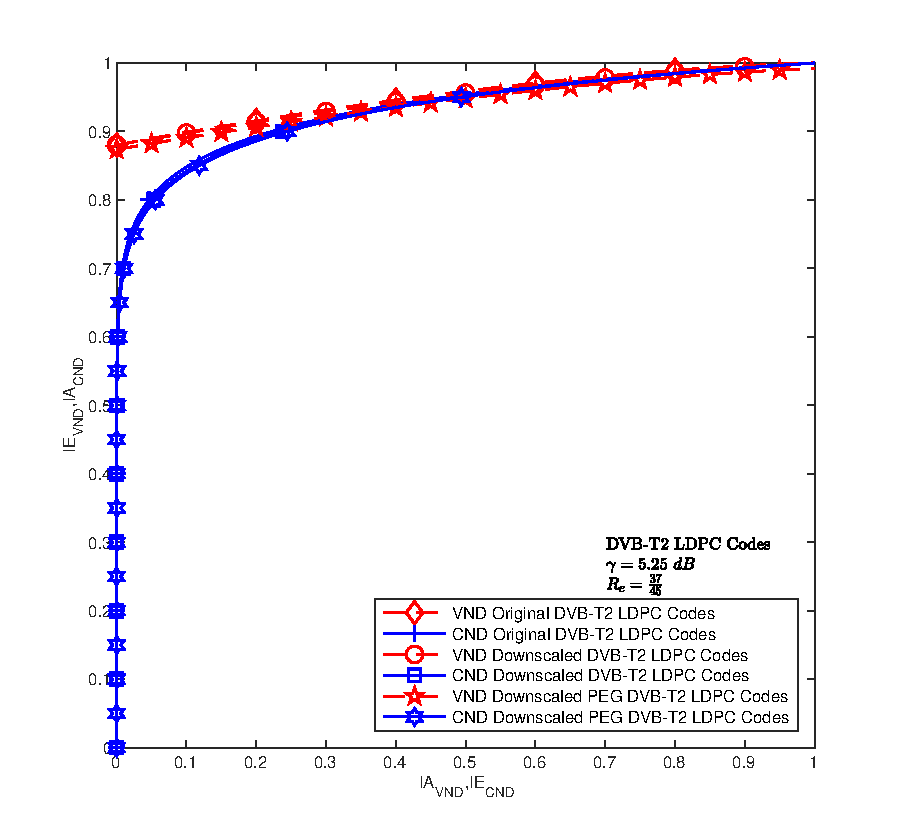
\includegraphics[width=0.85\textwidth]{pics/exit/56/56semua=snr5,25Ich=0,8804.pdf}
		\vspace{-1cm}
		\center (b)
	\end{minipage}
	%	\begin{minipage}{.5\linewidth}
	%		\hspace{-0.4 cm}
	%		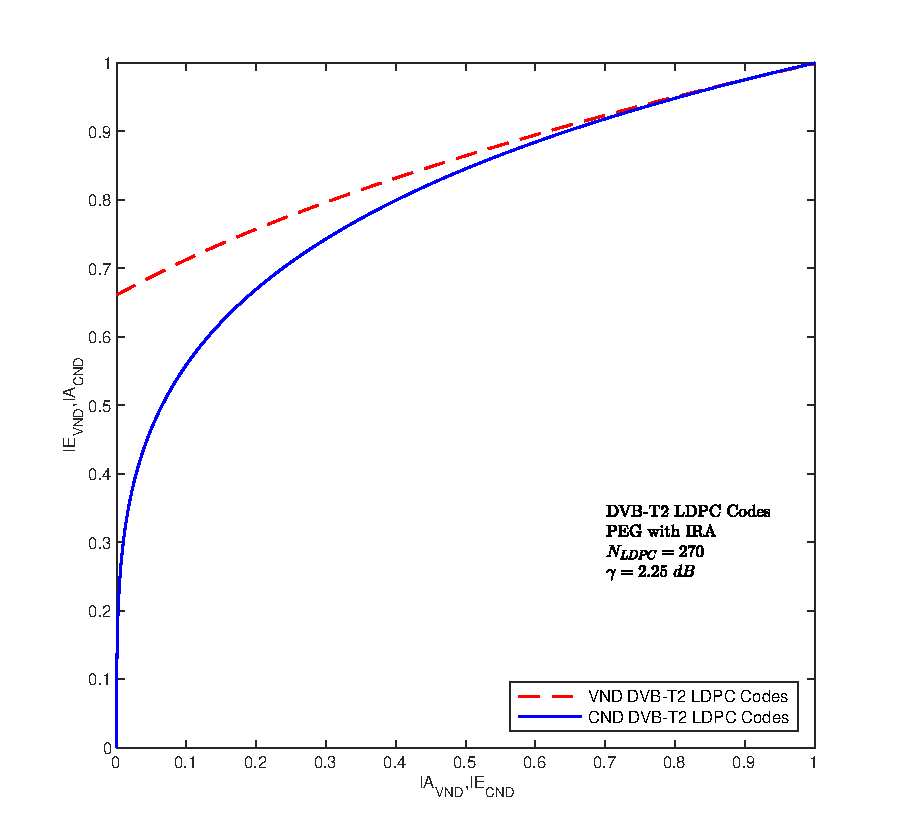
\includegraphics[width=3in]{pics/exit/12/12peg=snr2,25Ich=0,6613.pdf}
	%		\vspace{-1cm}
	%		\center (c)
	%	\end{minipage}
	\caption {Analisis EXIT \textit{chart} LDPC \textit{codes} DVB-T2 pada (a) $R_e=\frac{7}{9}$ dan (b) $R_e=\frac{37}{45}$, masing-masing, pada SNR $\gamma=4,5~dB$ dan $\gamma=5,25~dB$.}
	\label{gambar: exit737}
\end{figure}






%-----------------------------------------------------------------------------%

%EXIT
%\hspace{15cm}
%\begin{figure}
%	\centering
%	\hspace{-0.1 in}
%	\begin{minipage}{.5\linewidth}
%		\hspace{-0.5cm}
%		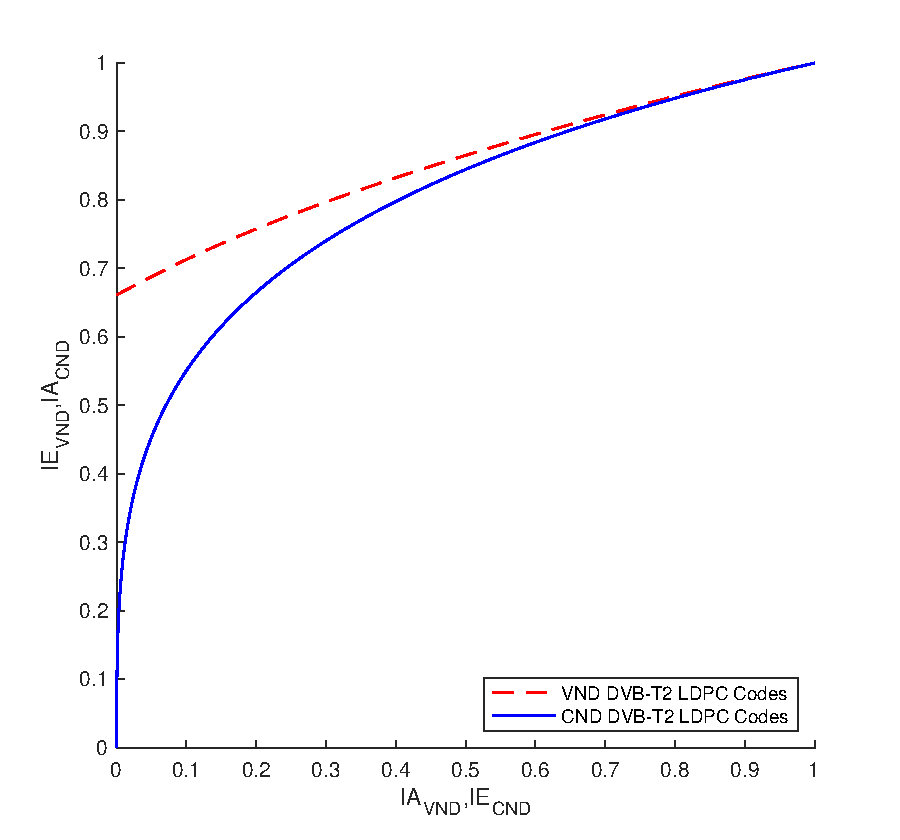
\includegraphics[width=3in]{pics/12/12asli=snr2,25Ich=0,6613.pdf}
%		\vspace{-1.25cm}
%		
%		\center (a)
%	\end{minipage}
%	\hfill 	\hspace{-0.1 in}
%	\begin{minipage}{.5\linewidth}
%%		\hspace{2.25 cm}
%		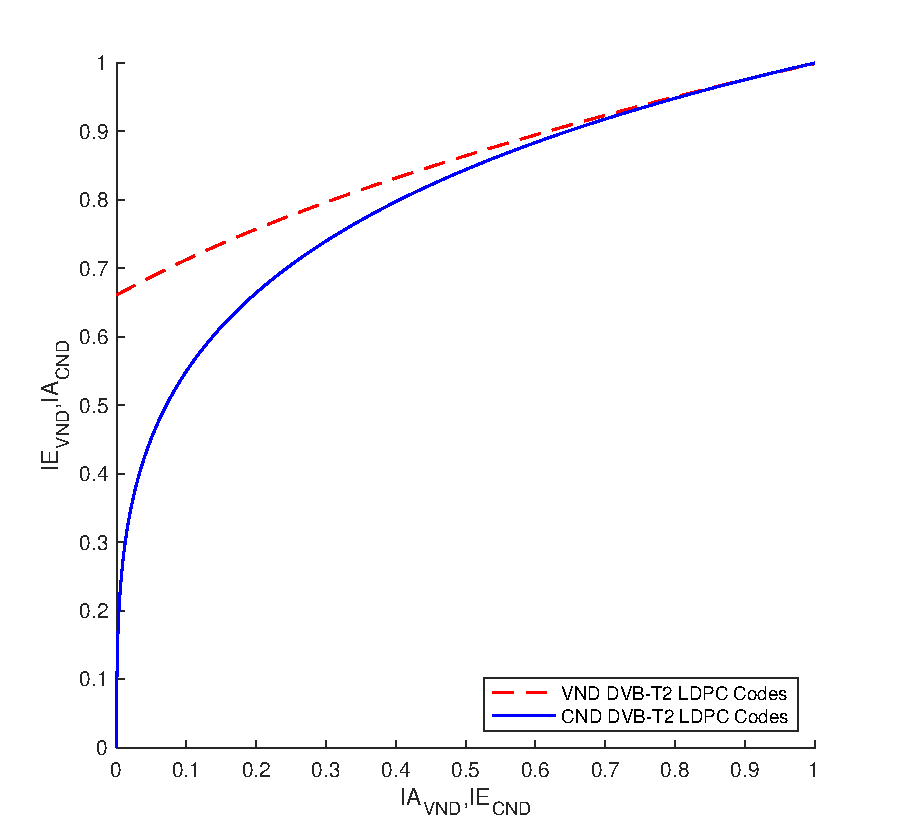
\includegraphics[width=3in]{pics/12/12ds=snr2,25Ich=0,6613.pdf}
%		\vspace{-1.15cm}
%		\center \hspace*{0.75cm}(b)
%	\end{minipage}
%	\begin{minipage}{.5\linewidth}
%		\hspace{-0.5cm}
%		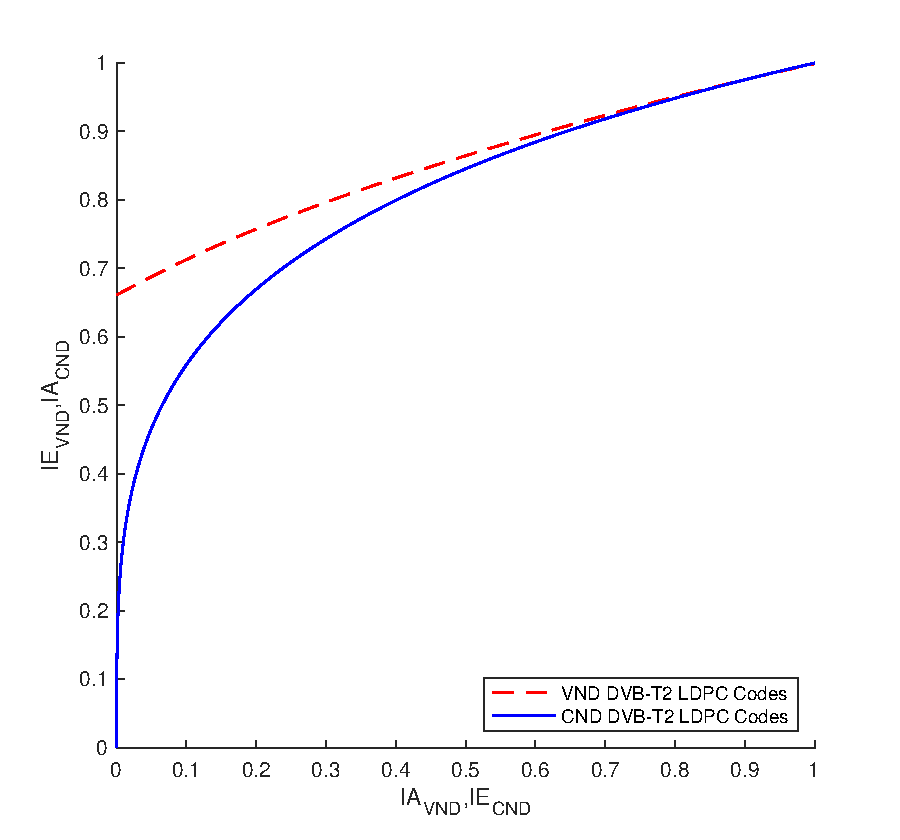
\includegraphics[width=3in]{pics/12/12peg=snr2,25Ich=0,6613.pdf}
%		\vspace{-1.25cm}
%		\center (c)
%	\end{minipage}
%	\hspace{-0.1 in}
%	\begin{minipage}{.5\linewidth}
%%		\hspace{2.25 cm}
%		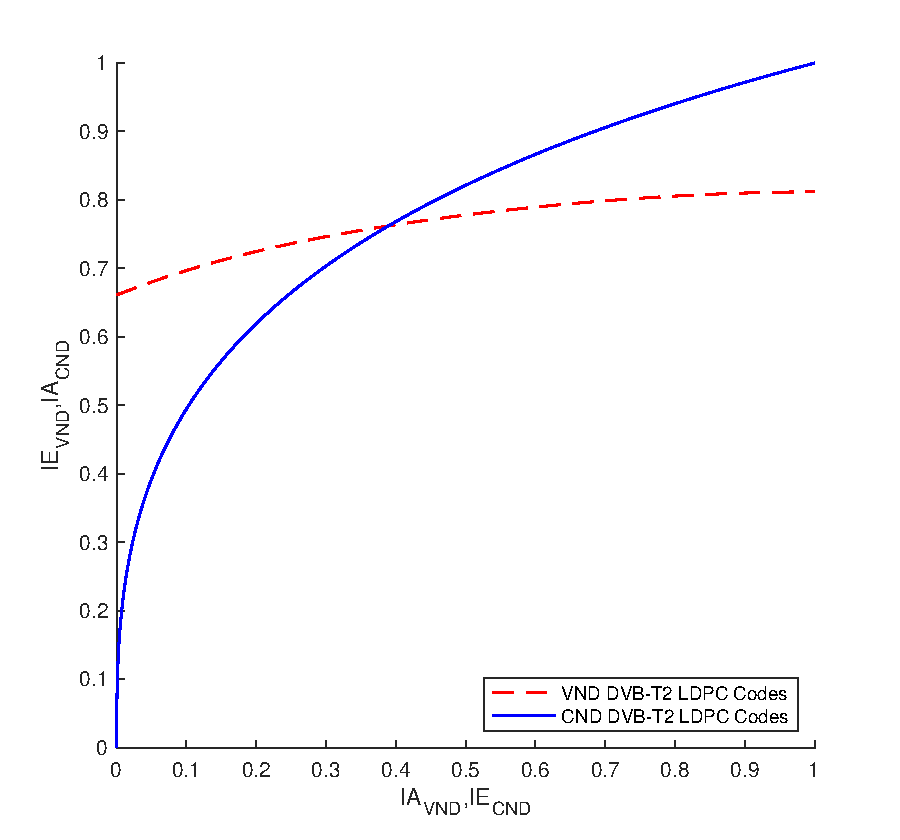
\includegraphics[width=3in]{pics/12/12pegLDGM=snr2,25Ich=0,6613.pdf}
%		\vspace{-1.25cm}
%		\center \hspace*{0.75cm}(d)
%	\end{minipage}
%	\caption {Analisis EXIT \textit{Chart} LDPC \textit{codes} DVB-T2 $R_e=\frac{4}{9}$ dengan: (a)  $N_{LDPC}=16200$, (b) $N_{LDPC}=270$ menggunakan metode \textit{downscaled}, (c) $N_{LDPC}=270$ menggunakan PEG dengan \textit{accumulator}, dan (d) $N_{LDPC} = 270 $ menggunakan PEG dengan LDGM.}
%	\label{gambar: exit49}
%\end{figure}



%
%\begin{figure}
%	\centering
%	\hspace{-0.2 in}
%	\begin{minipage}{.5\linewidth}
%		\hspace{-0.4 cm}
%		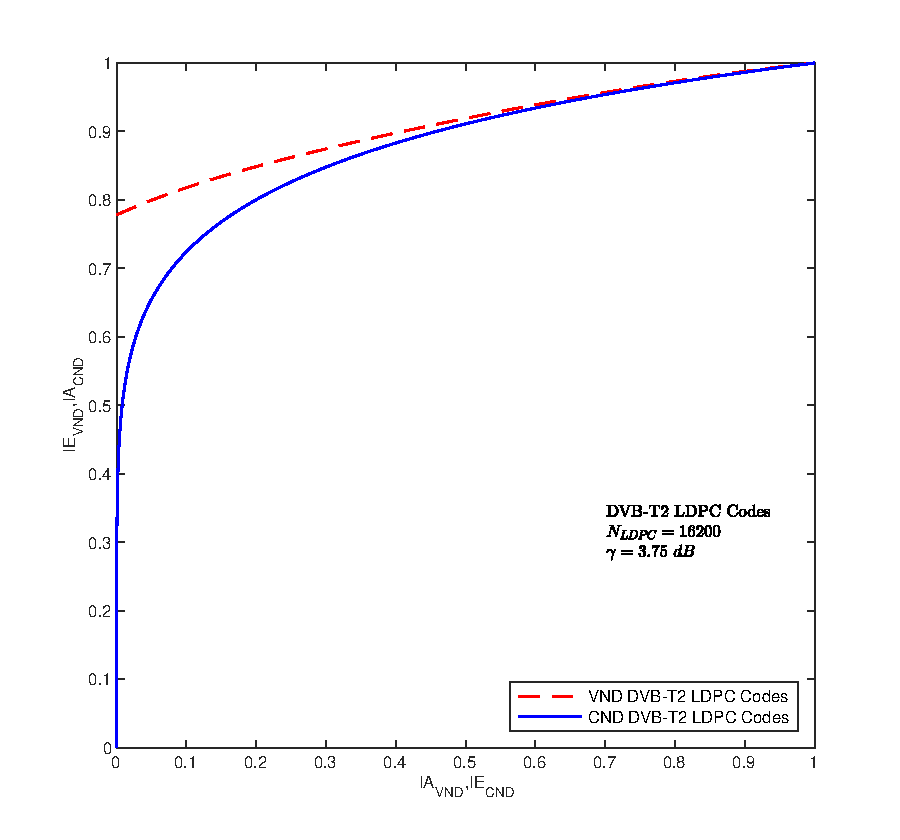
\includegraphics[width=3in]{pics/exit/35/35asli=snr3,75Ich=0,7786.pdf}
%		\vspace{-1cm}
%		
%		\center (a)
%	\end{minipage}
%	\hfill
%	\begin{minipage}{.5\linewidth}
%		\hspace{-0.4 cm}
%		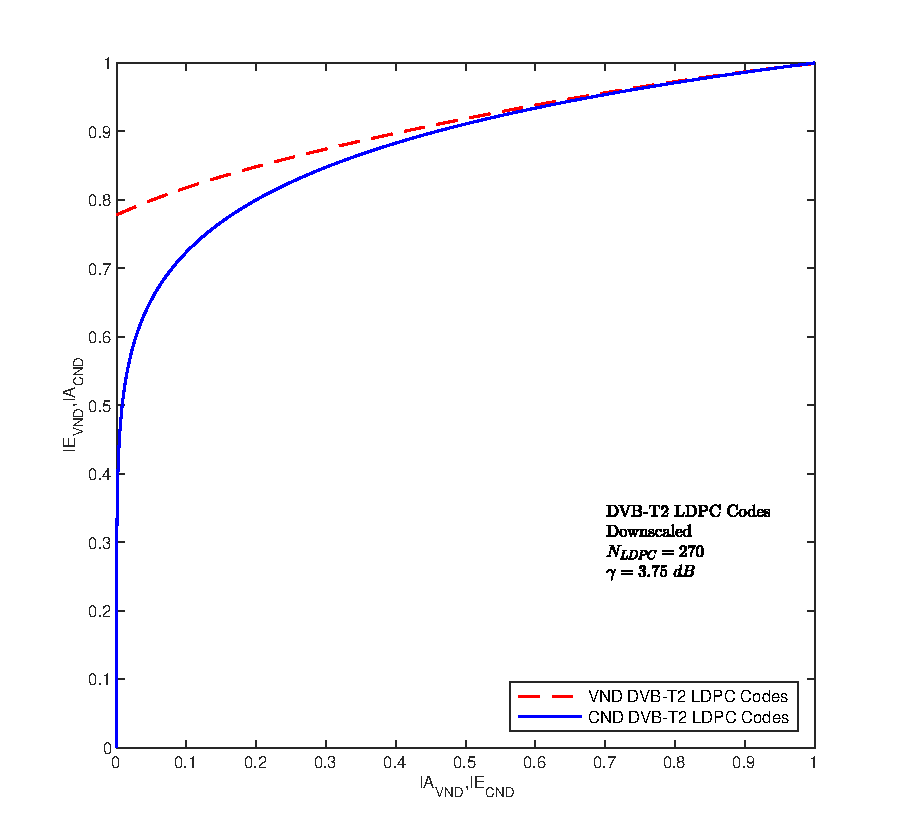
\includegraphics[width=3in]{pics/exit/35/35ds=snr3,75Ich=0,7786.pdf}
%		\vspace{-1cm}
%		\center (b)
%	\end{minipage}
%	\begin{minipage}{.5\linewidth}
%		\hspace{-0.4 cm}
%		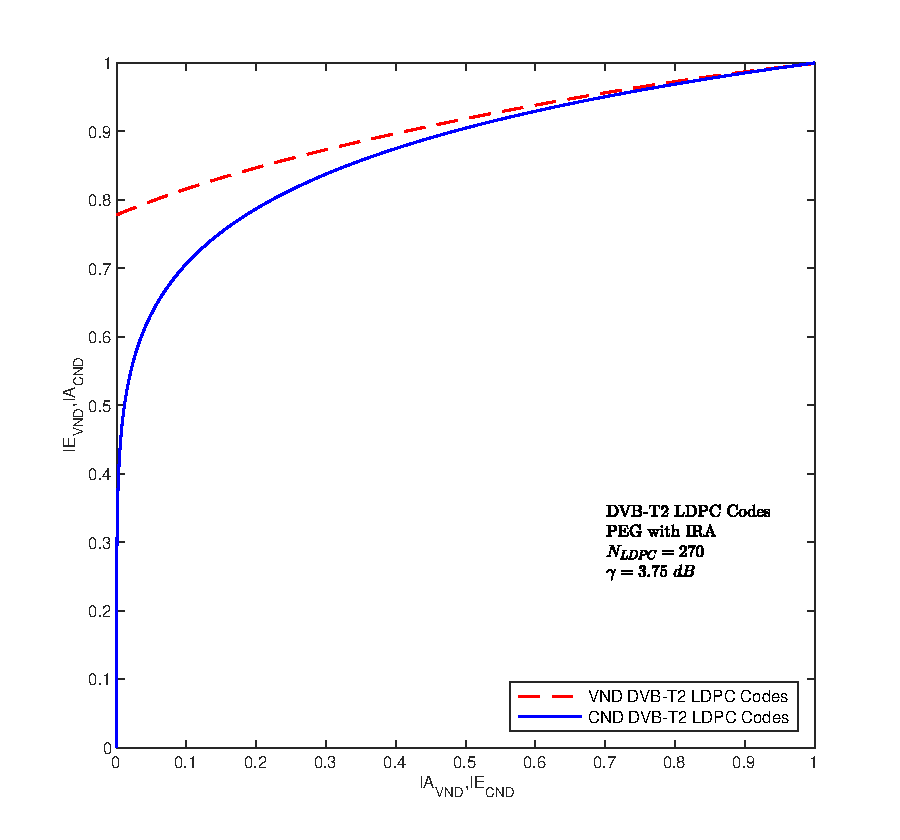
\includegraphics[width=3in]{pics/exit/35/35peg=snr3,75Ich=0,7786.pdf}
%		\vspace{-1cm}
%		\center (c)
%	\end{minipage}
%%		\caption {Analisis EXIT \textit{Chart} LDPC \textit{codes} DVB-T2 $R_e=\frac{3}{5}$ dengan: (a)  $N_{LDPC}=16200$, (b) $N_{LDPC}=270$ menggunakan metode \textit{downscaled}, dan (c) $N_{LDPC}=270$ menggunakan PEG.}
%	\caption {Analisis EXIT \textit{Chart} LDPC \textit{codes} DVB-T2 $R_e=\frac{3}{5}$.}
%	\label{gambar: exit35}
%\end{figure}
%
%\begin{figure}
%	\centering
%	\hspace{-0.2 in}
%	\begin{minipage}{.5\linewidth}
%		\hspace{-0.4 cm}
%		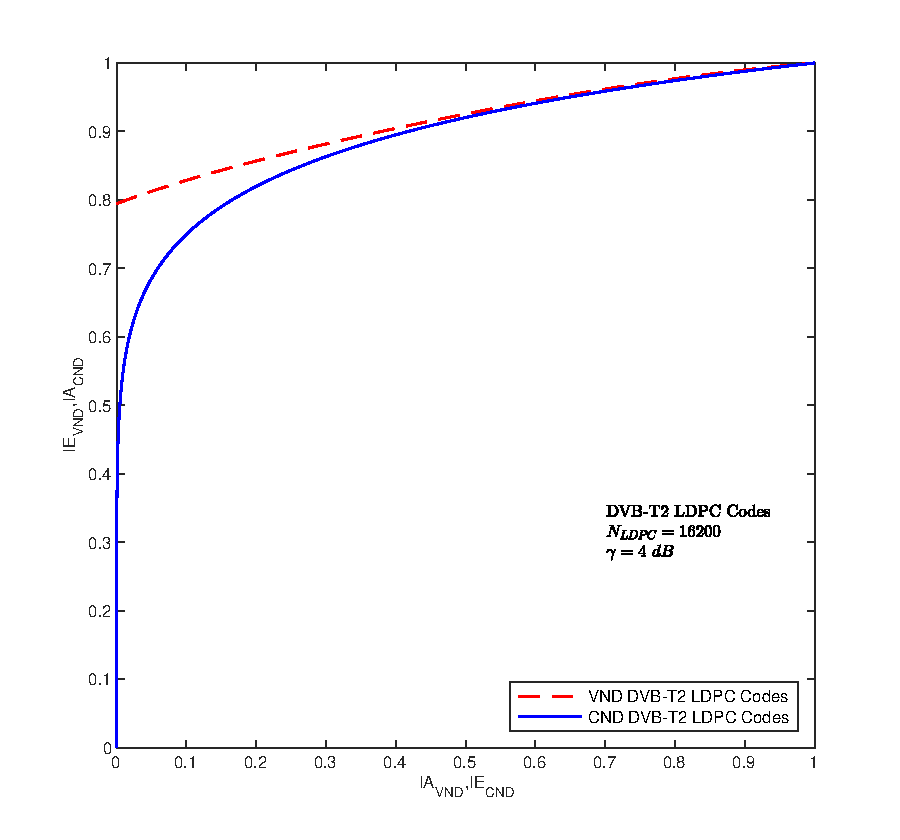
\includegraphics[width=3in]{pics/exit/23/23asli=snr4Ich=0,795.pdf}
%		\vspace{-1cm}
%		
%		\center (a)
%	\end{minipage}
%	\hfill
%	\begin{minipage}{.5\linewidth}
%		\hspace{-0.4 cm}
%		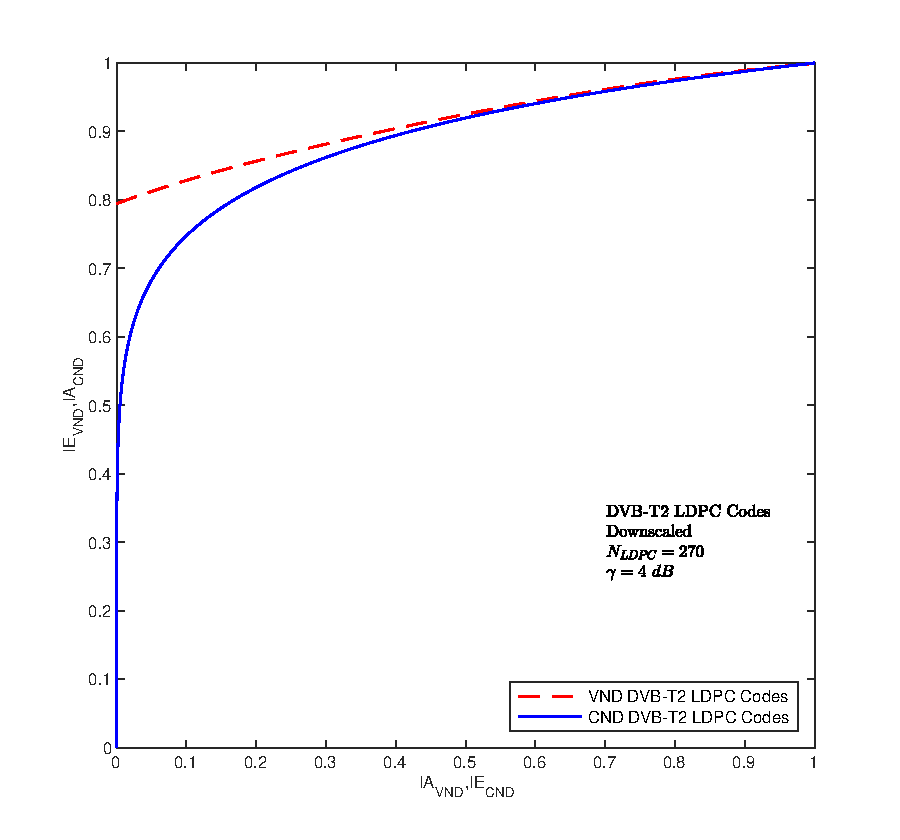
\includegraphics[width=3in]{pics/exit/23/23ds=snr4Ich=0,795.pdf}
%		\vspace{-1cm}
%		\center (b)
%	\end{minipage}
%	\begin{minipage}{.5\linewidth}
%		\hspace{-0.4 cm}
%		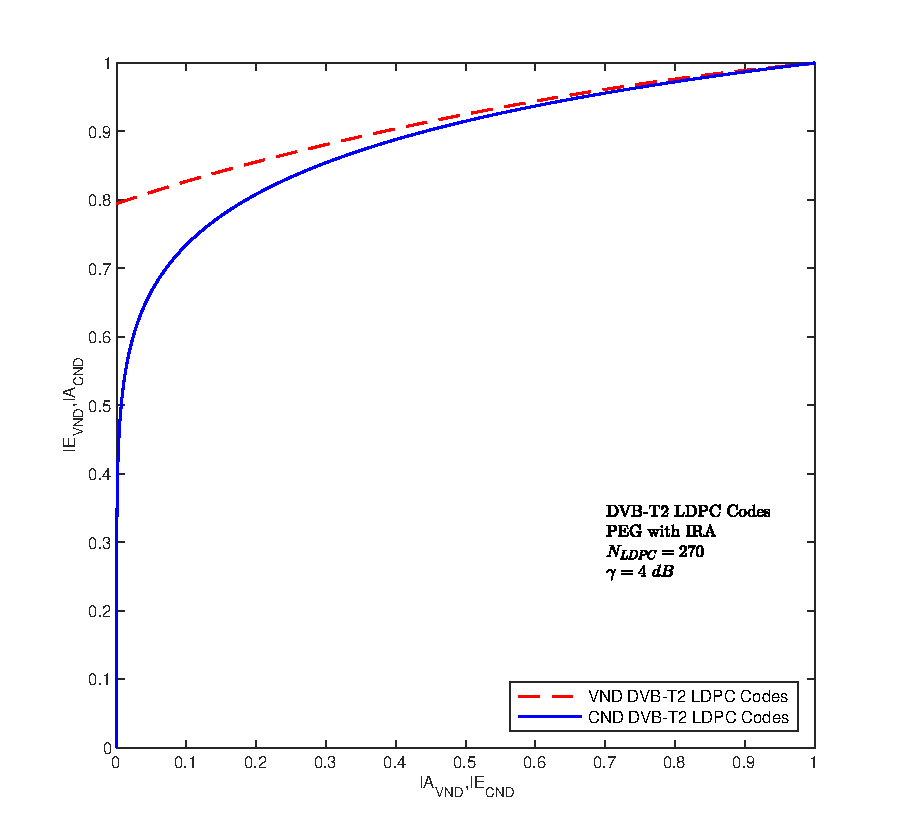
\includegraphics[width=3in]{pics/exit/23/23peg=snr4Ich=0,795.pdf}
%		\vspace{-1cm}
%		\center (c)
%	\end{minipage}
%%		\caption {Analisis EXIT \textit{Chart} LDPC \textit{codes} DVB-T2 $R_e=\frac{2}{3}$ dengan: (a)  $N_{LDPC}=16200$, (b) $N_{LDPC}=270$ menggunakan metode \textit{downscaled}, dan (c) $N_{LDPC}=270$ menggunakan PEG.}
%			\caption {Analisis EXIT \textit{Chart} LDPC \textit{codes} DVB-T2 $R_e=\frac{2}{3}$.}
%	\label{gambar: exit23}
%\end{figure}
%
%\begin{figure}
%	\centering
%	\hspace{-0.2 in}
%	\begin{minipage}{.5\linewidth}
%		\hspace{-0.4 cm}
%		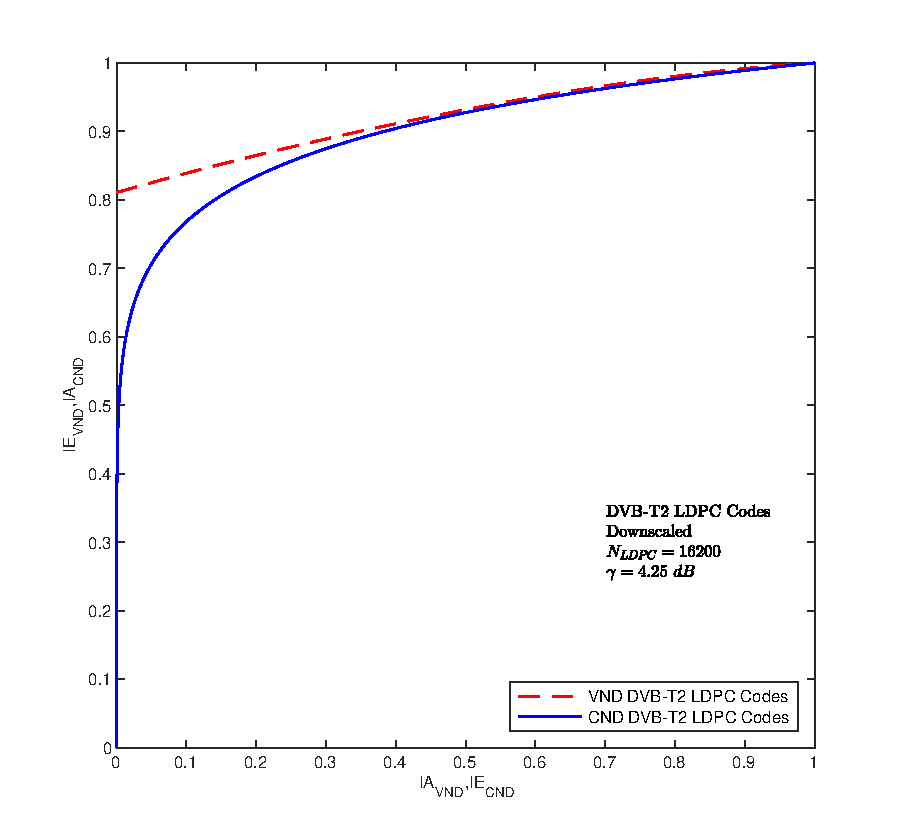
\includegraphics[width=3in]{pics/exit/34/34asli=snr4,25Ich=0,8113.pdf}
%		\vspace{-1cm}
%		
%		\center (a)
%	\end{minipage}
%	\hfill
%	\begin{minipage}{.5\linewidth}
%		\hspace{-0.4 cm}
%		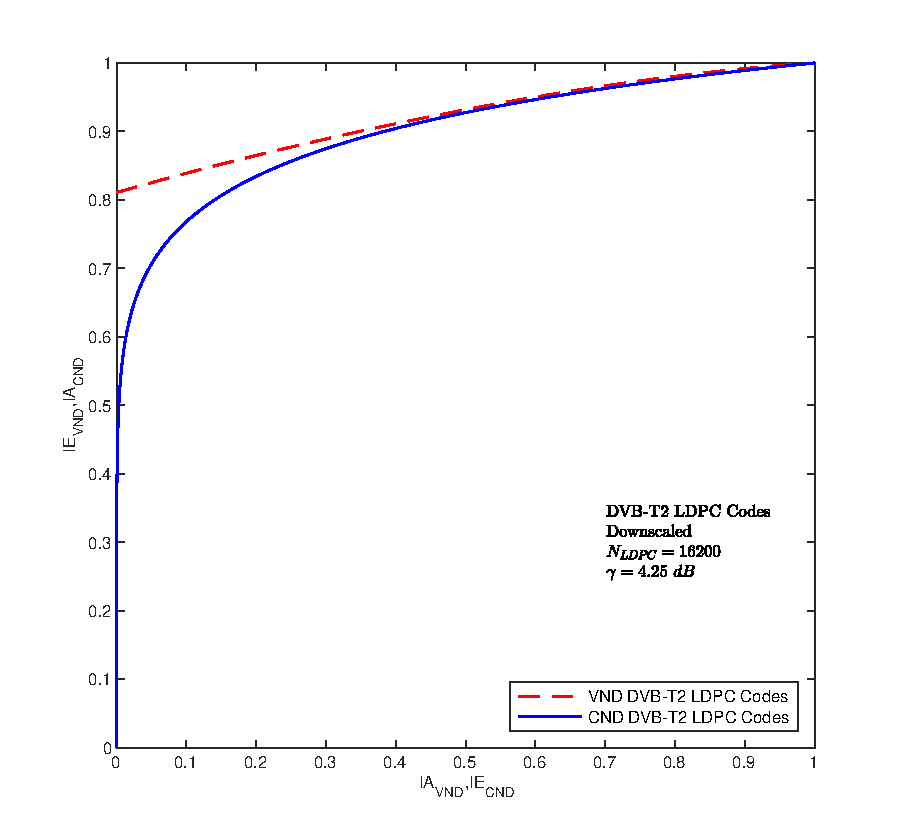
\includegraphics[width=3in]{pics/exit/34/34asli=snr4,25Ich=0,8113.pdf}
%		\vspace{-1cm}
%		\center (b)
%	\end{minipage}
%	\begin{minipage}{.5\linewidth}
%		\hspace{-0.4 cm}
%		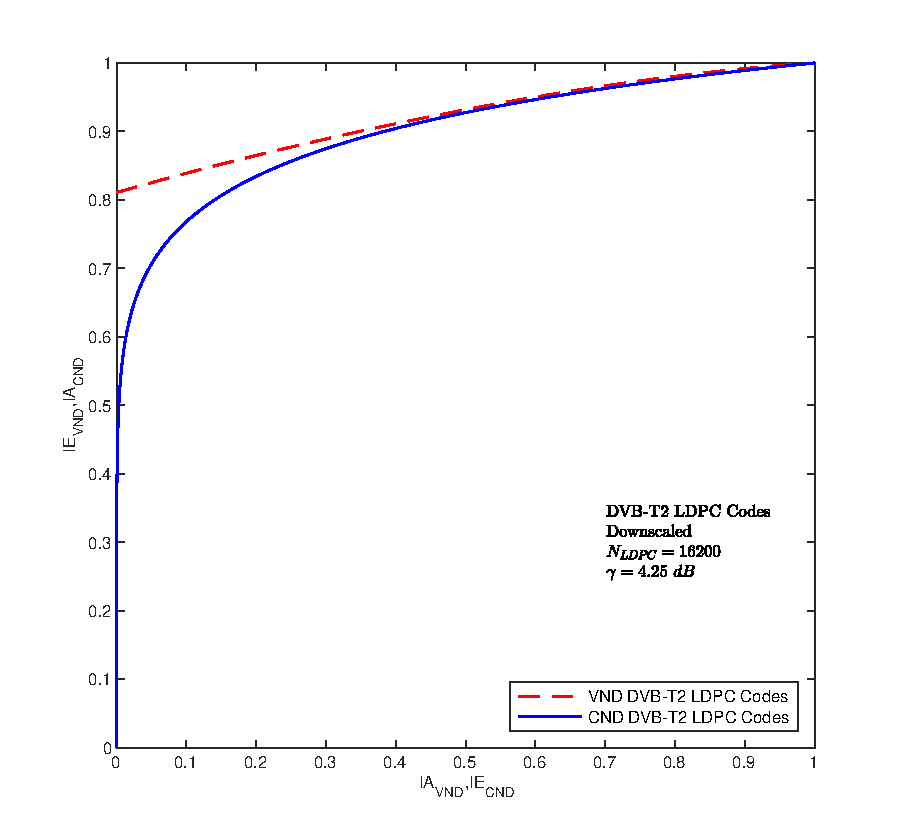
\includegraphics[width=3in]{pics/exit/34/34asli=snr4,25Ich=0,8113.pdf}
%		\vspace{-1cm}
%		\center (c)
%	\end{minipage}
%%		\caption {Analisis EXIT \textit{Chart} LDPC \textit{codes} DVB-T2 $R_e=\frac{11}{15}$ dengan: (a)  $N_{LDPC}=16200$, (b) $N_{LDPC}=270$ menggunakan metode \textit{downscaled}, dan (c) $N_{LDPC}=270$ menggunakan PEG.}
%		\caption {Analisis EXIT \textit{Chart} LDPC \textit{codes} DVB-T2 $R_e=\frac{11}{15}$.}
%	\label{gambar: exit1115}
%\end{figure}
%
%\begin{figure}
%	\centering
%	\hspace{-0.2 in}
%	\begin{minipage}{.5\linewidth}
%		\hspace{-0.4 cm}
%		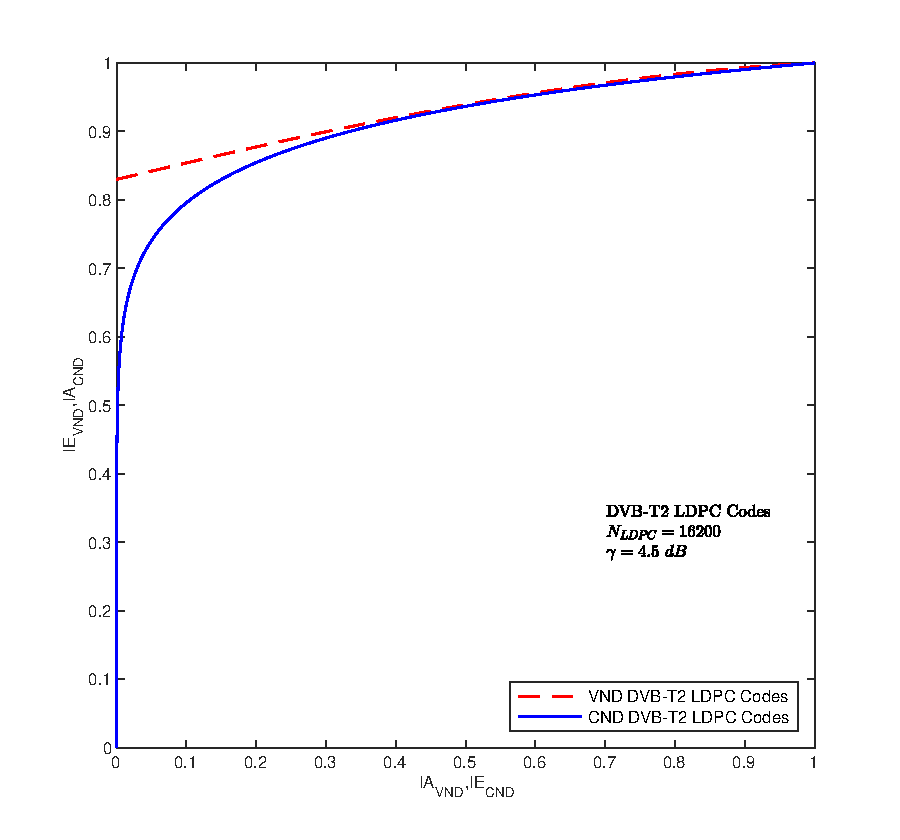
\includegraphics[width=3in]{pics/exit/45/45asli=snr4,5Ich=0,8303.pdf}
%		\vspace{-1cm}
%		
%		\center (a)
%	\end{minipage}
%	\hfill
%	\begin{minipage}{.5\linewidth}
%		\hspace{-0.4 cm}
%		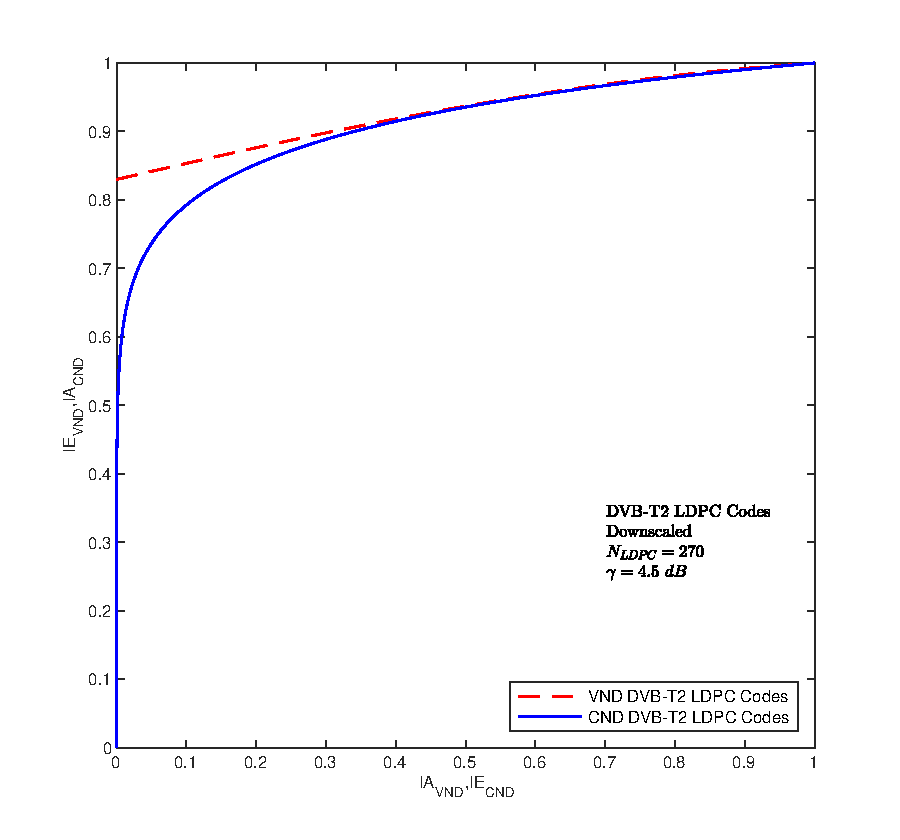
\includegraphics[width=3in]{pics/exit/45/45ds=snr4,5Ich=0,8303.pdf}
%		\vspace{-1cm}
%		\center (b)
%	\end{minipage}
%	\begin{minipage}{.5\linewidth}
%		\hspace{-0.4 cm}
%		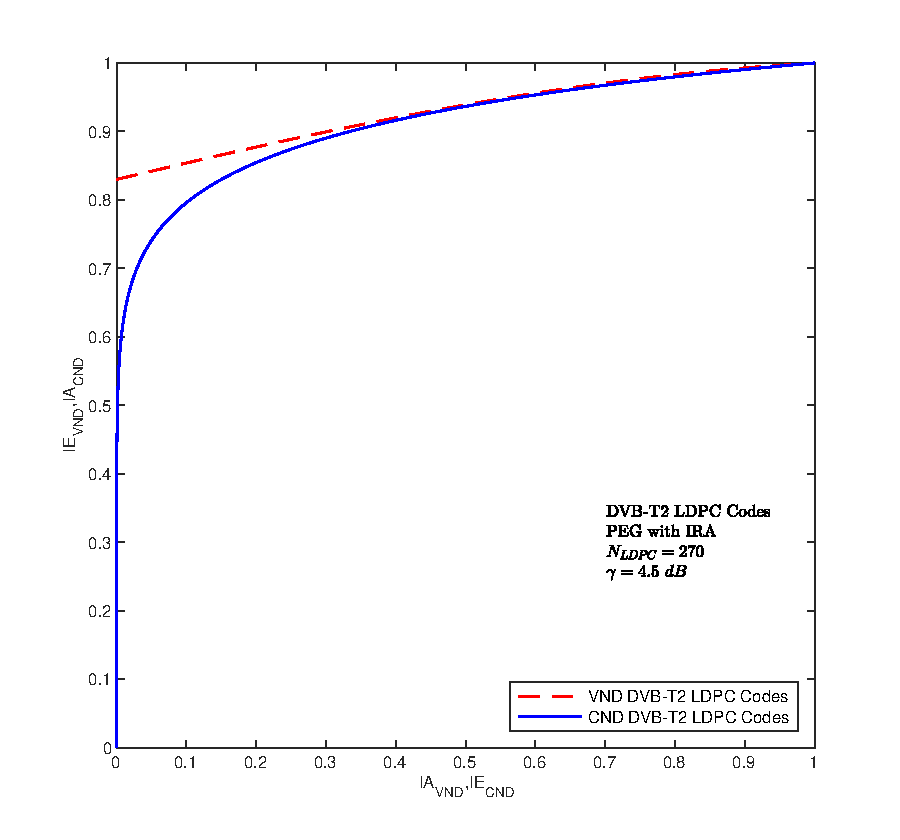
\includegraphics[width=3in]{pics/exit/45/45peg=snr4,5Ich=0,8303.pdf}
%		\vspace{-1cm}
%		\center (c)
%	\end{minipage}
%%		\caption {Analisis EXIT \textit{Chart} LDPC \textit{codes} DVB-T2 $R_e=\frac{7}{9}$ dengan: (a)  $N_{LDPC}=16200$, (b) $N_{LDPC}=270$ menggunakan metode \textit{downscaled}, dan (c) $N_{LDPC}=270$ menggunakan PEG.}
%		\caption {Analisis EXIT \textit{Chart} LDPC \textit{codes} DVB-T2 $R_e=\frac{7}{9}$.}
%	\label{gambar: exit79}
%\end{figure}
%
%\begin{figure}
%	\centering
%	\hspace{-0.2 in}
%	\begin{minipage}{.5\linewidth}
%		\hspace{-0.4 cm}
%		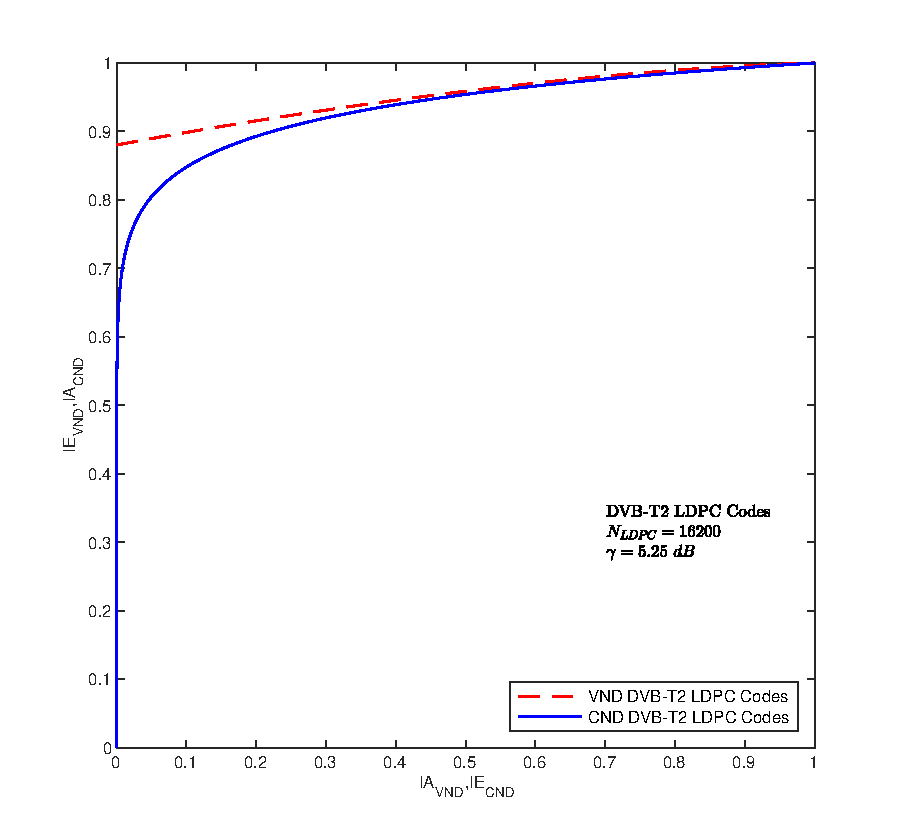
\includegraphics[width=3in]{pics/exit/56/56asli=snr5,25Ich=0,8804.pdf}
%		\vspace{-1cm}
%		
%		\center (a)
%	\end{minipage}
%	\hfill
%	\begin{minipage}{.5\linewidth}
%		\hspace{-0.4 cm}
%		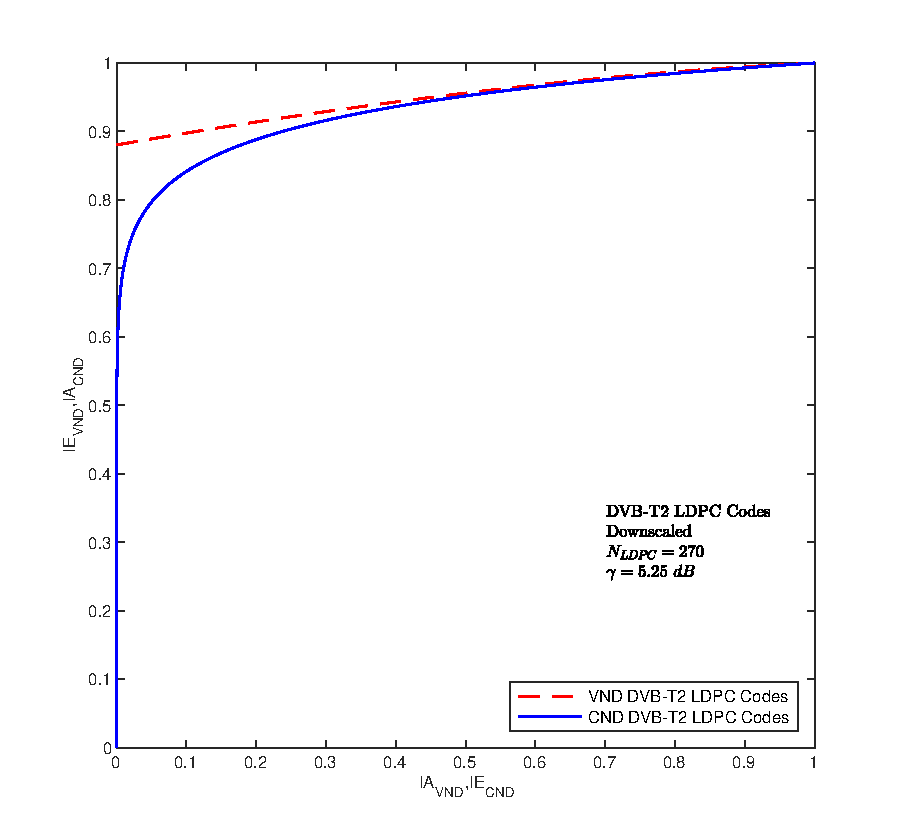
\includegraphics[width=3in]{pics/exit/56/56ds=snr5,25Ich=0,8804.pdf}
%		\vspace{-1cm}
%		\center (b)
%	\end{minipage}
%	\begin{minipage}{.5\linewidth}
%		\hspace{-0.4 cm}
%		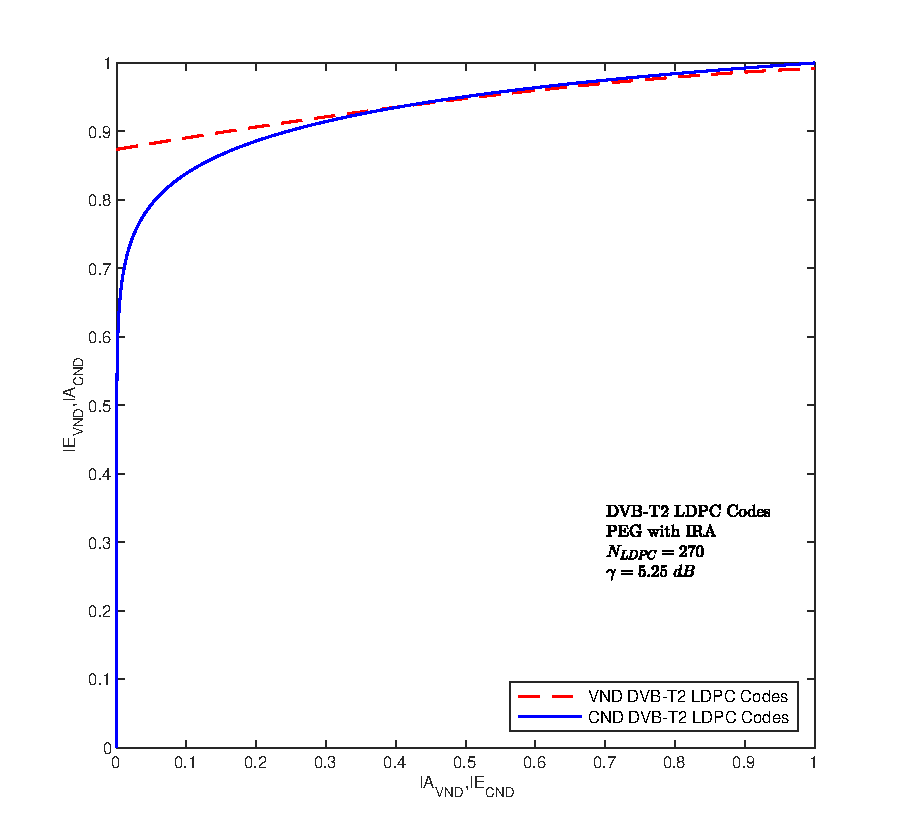
\includegraphics[width=3in]{pics/exit/56/56peg=snr5,25Ich=0,8804.pdf}
%		\vspace{-1cm}
%		\center (c)
%	\end{minipage}
%%	\caption {Analisis EXIT \textit{Chart} LDPC \textit{codes} DVB-T2 $R_e=\frac{37}{45}$ dengan: (a)  $N_{LDPC}=16200$, (b) $N_{LDPC}=270$ menggunakan metode \textit{downscaled}, dan (c) $N_{LDPC}=270$ menggunakan PEG.}
%		\caption {Analisis EXIT \textit{Chart} LDPC \textit{codes} DVB-T2 $R_e=\frac{37}{45}$.}
%\label{gambar: exit3745}
%\end{figure}










% Gambar \ref{gambar: exit49} menunjukkan perbandingan EXIT \textit{chart} antara original, \textit{downscaled}, dan \textit{downscaled} menggunakan PEG DVB-T2 LDPC \textit{codes} dengan code rate $R_e=\frac{4}{9}$ pada SNR $\gamma=2,25$. Gambar \ref{gambar: exit35} menunjukkan perbandingan EXIT \textit{chart} antara original, \textit{downscaled}, dan \textit{downscaled} menggunakan PEG DVB-T2 LDPC \textit{codes} dengan code rate $R_e=\frac{3}{5}$ pada SNR $\gamma=3,75$. Gambar \ref{gambar: exit23} menunjukkan perbandingan EXIT \textit{chart} antara original, \textit{downscaled}, dan \textit{downscaled} menggunakan PEG DVB-T2 LDPC \textit{codes} dengan code rate $R_e=\frac{2}{3}$ pada SNR $\gamma=4$. Gambar \ref{gambar: exit1115} menunjukkan perbandingan EXIT \textit{chart} antara original, \textit{downscaled}, dan \textit{downscaled} menggunakan PEG DVB-T2 LDPC \textit{codes} dengan code rate $R_e=\frac{11}{15}$ pada SNR $\gamma=4,25$. Gambar \ref{gambar: exit79} menunjukkan perbandingan EXIT \textit{chart} antara original, \textit{downscaled}, dan \textit{downscaled} menggunakan PEG DVB-T2 LDPC \textit{codes} dengan code rate $R_e=\frac{7}{9}$ pada SNR $\gamma=4,5$. Gambar \ref{gambar: exit3745} menunjukkan perbandingan EXIT \textit{chart} antara original, \textit{downscaled}, dan \textit{downscaled} menggunakan PEG DVB-T2 LDPC \textit{codes} dengan code rate $R_e=\frac{37}{45}$ pada SNR $\gamma=5,25$.

 %-----------------------------------------------------------------------------%

\section{Analisis Kinerja BER}
Tugas Akhir ini mengevaluasi kinerja BER dari LDPC \textit{codes} DVB-T2 dengan $N_{LDPC}=16200$, \textit{downscaled} LDPC \textit{codes} DVB-T2 dengan $N_{LDPC}=270$, \textit{downscaled} LDPC \textit{codes} DVB-T2 menggunakan PEG dengan \textit{accumulator}, dan \textit{downscaled} LDPC \textit{codes} DVB-T2 menggunakan PEG dengan LDGM pada kanal AWGN dan \textit{channel model} DVB-T2 Indonesia.
% yang direpresentasikan oleh \textit{channel model} DVB-T2 Kota Bandung.


%\begin{figure}
%	\centering
%	\hspace{ -0.1in}
%	\begin{minipage}{.5\linewidth}
%		\hspace{-1.15cm}
%		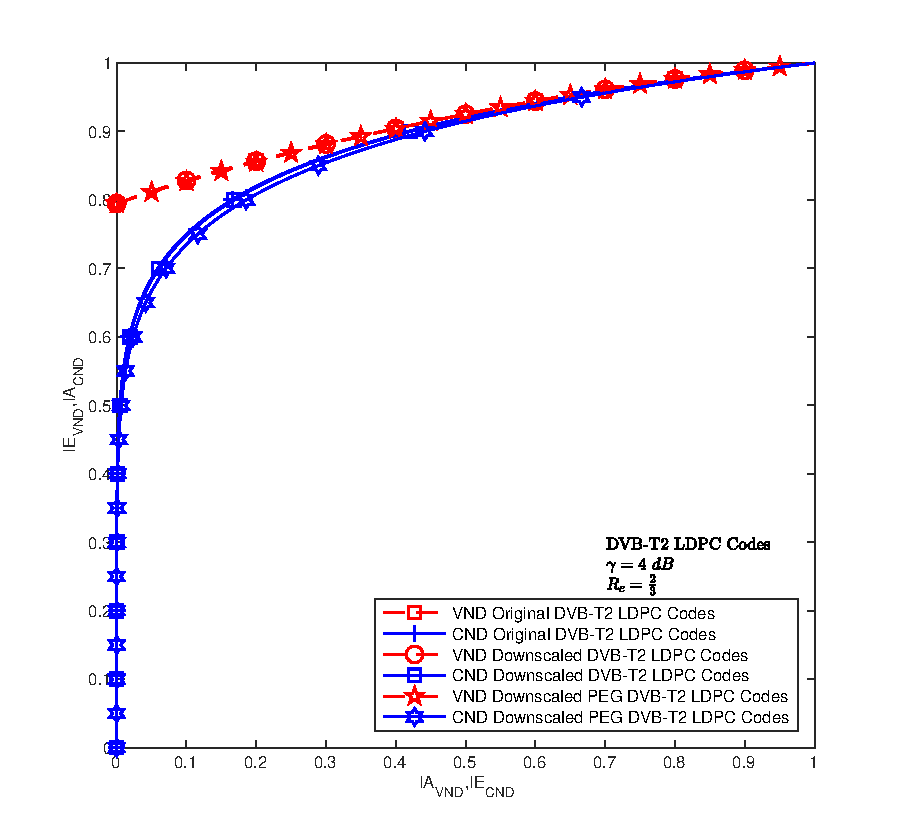
\includegraphics[width=3.5in]{pics/exit/23/23semua=snr4Ich=0,795.pdf}
%		\vspace{-1.5cm}
%		
%		\center (a)
%	\end{minipage}
%	\hfill 	\hspace{ -0.1in}
%	\begin{minipage}{.5\linewidth}
%%		\hspace{2.25 cm}
%		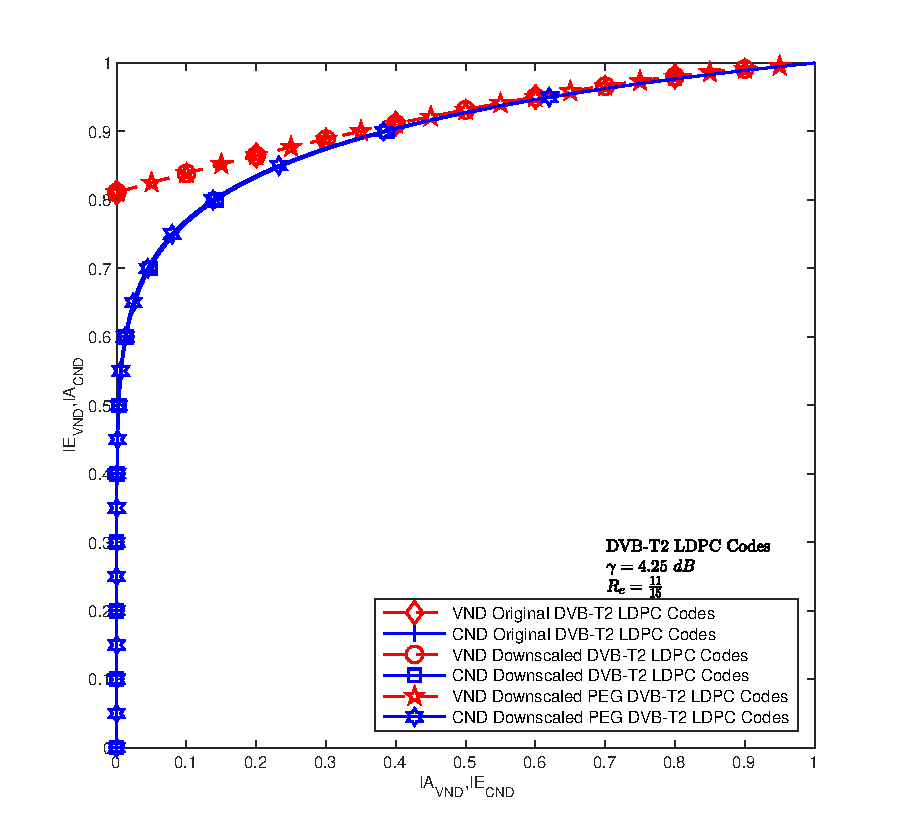
\includegraphics[width=3.5in]{pics/exit/34/34semua=snr4,25Ich=0,8113.pdf}
%		
%		\vspace{-0.95cm}
%		\center \hspace*{2.25cm}(b)
%	\end{minipage}
%	
%	\begin{minipage}{.5\linewidth}
%		\hspace{-1.25cm}
%		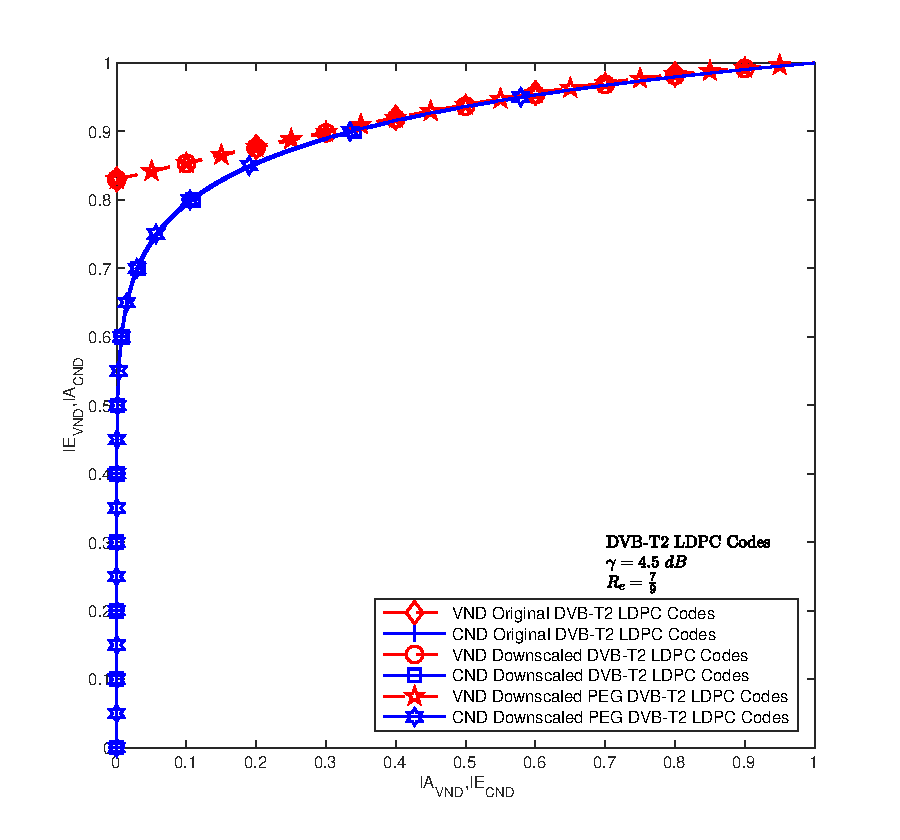
\includegraphics[width=3.5in]{pics/exit/45/45semua=snr4,5Ich=0,8303.pdf}
%		\vspace{-1.5cm}
%		\center (c)
%	\end{minipage}
%	\hfill \hspace{-0.1 in}
%	\begin{minipage}{.5\linewidth}
%%		\hspace{2.25 cm}
%		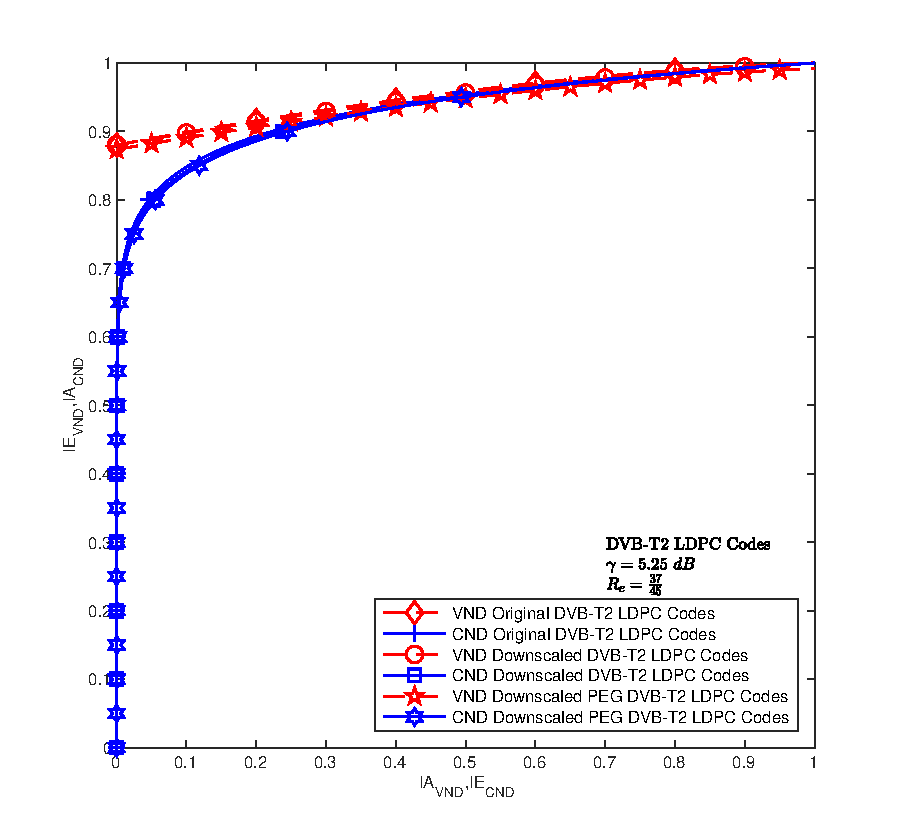
\includegraphics[width=3.5in]{pics/exit/56/56semua=snr5,25Ich=0,8804.pdf}
%		\vspace{-1.5cm}
%		\center \hspace*{2.25cm}(d)
%	\end{minipage}
%	\caption {Analisis EXIT \textit{chart} LDPC \textit{codes} DVB-T2 pada (a) $R_e=\frac{2}{3}$, (b) $R_e=\frac{11}{15}$, (c) $R_e=\frac{7}{9}$, dan (d) $R_e=\frac{37}{45}$.}
%	\label{gambar: exit4}
%\end{figure}


%\begin{figure}
%	\centering
%	\hspace{-0.2 in}
%	\begin{minipage}{.5\linewidth}
%		\hspace{-0.4 cm}
%		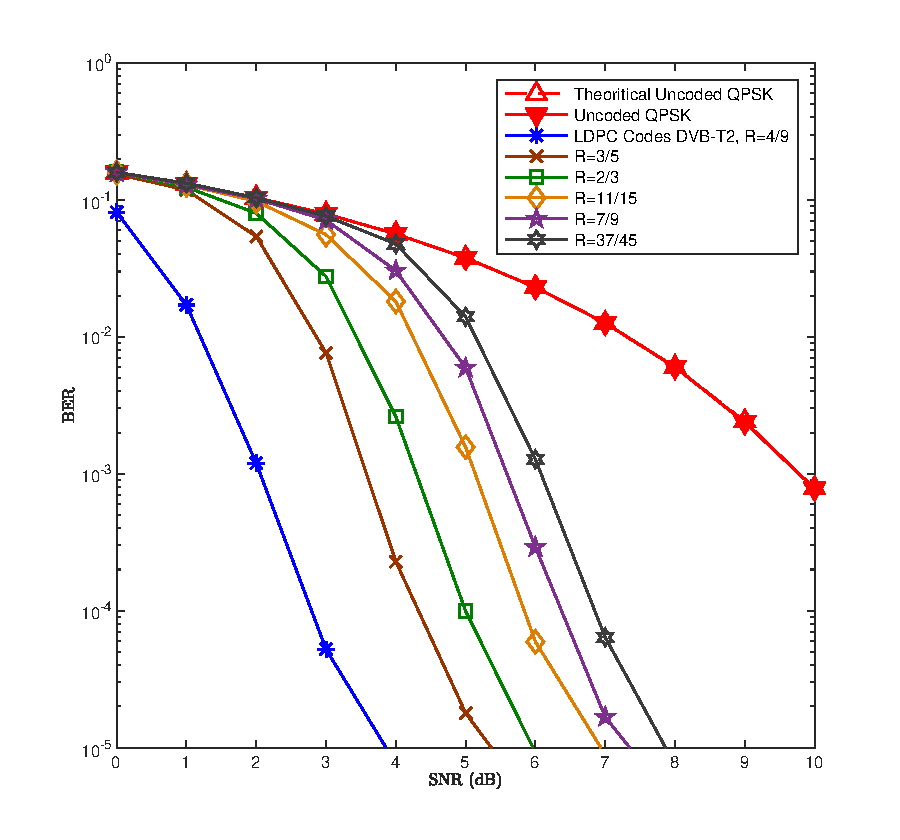
\includegraphics[width=3in]{hasildsfix.pdf}
%		\vspace{-1cm}
%		
%		\center (a)
%	\end{minipage}
%	\hfill
%	\begin{minipage}{.5\linewidth}
%		\hspace{-0.4 cm}
%		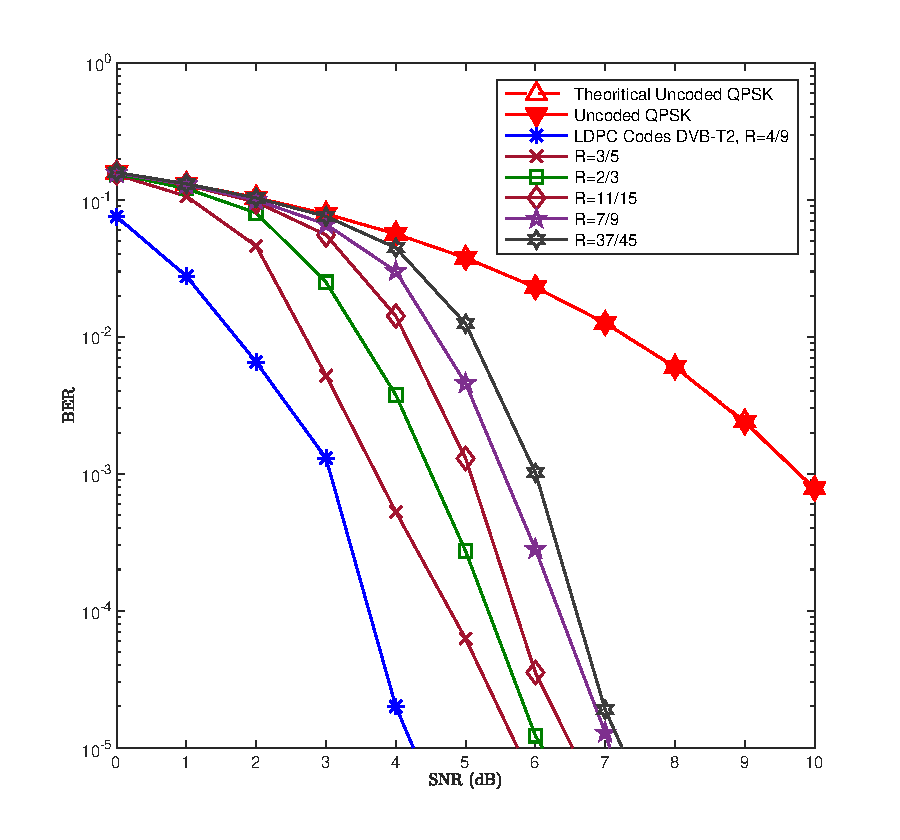
\includegraphics[width=3in]{hasilpegawgn.pdf}
%		\vspace{-1cm}
%		\center (b)
%	\end{minipage}
%	\hspace{-0.8 in}
%	\begin{minipage}{.5\linewidth}
%		\hspace{-0.4 cm}
%		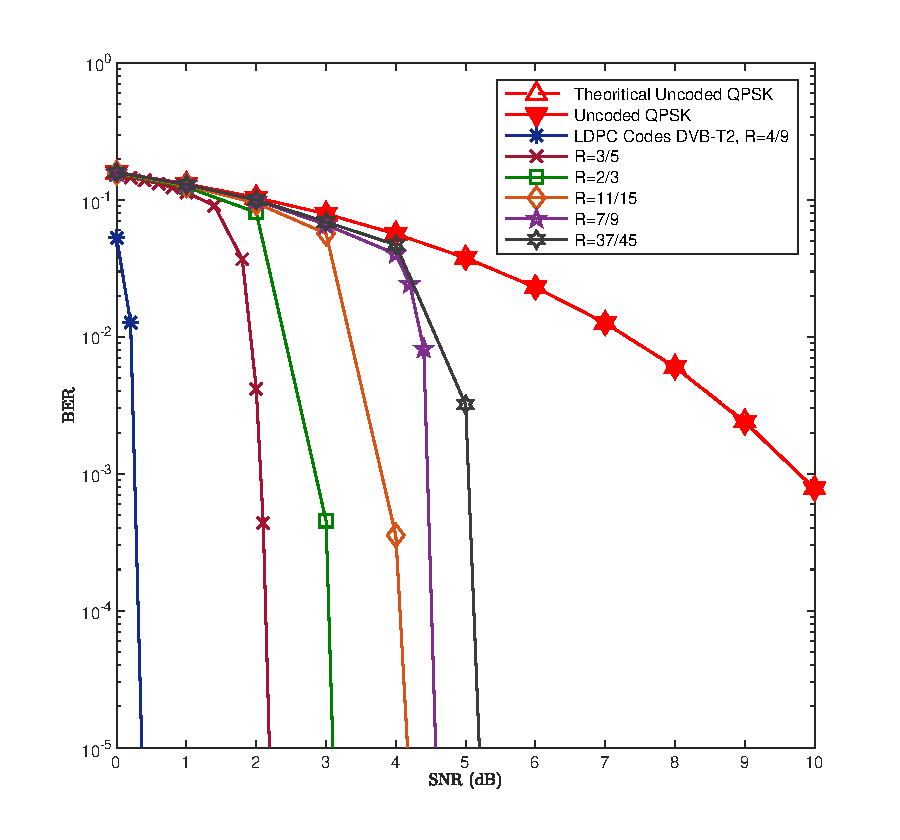
\includegraphics[width=3in]{hasiloriAWGN.pdf}
%		\vspace{-1cm}
%		\center (c)
%	\end{minipage}
%	\begin{minipage}{.5\linewidth}
%	\hspace{2.25 cm}
%	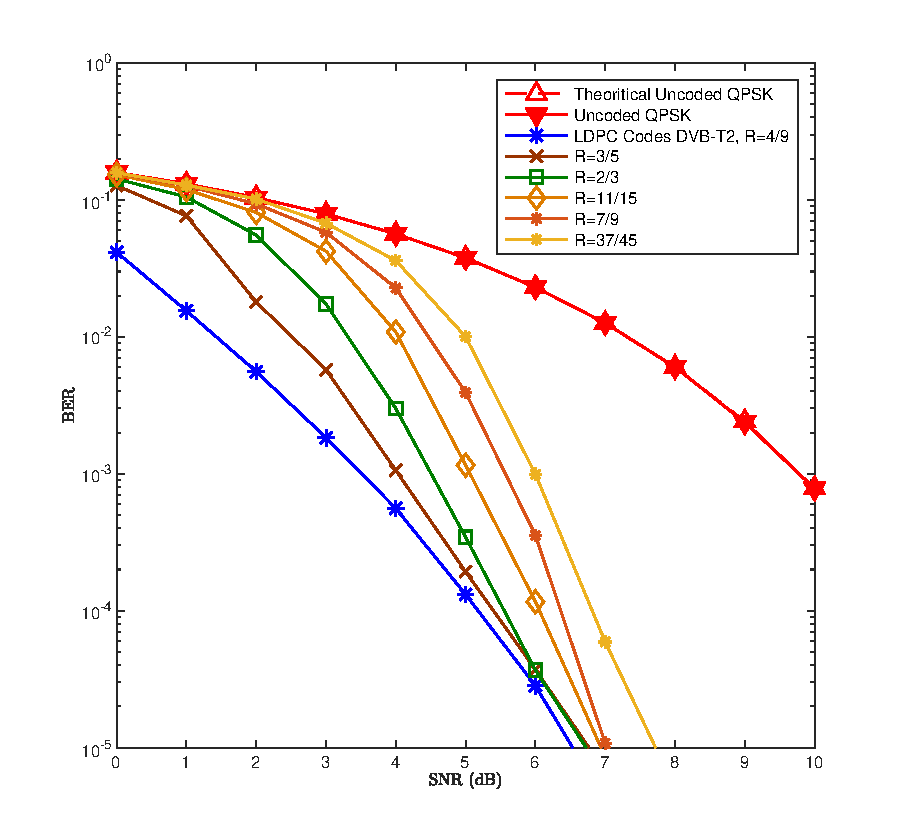
\includegraphics[width=3in]{hasilpegawgnfixLDGM.pdf}
%	\vspace{-0.5cm}
%	\center (c)
%\end{minipage}
%	\caption {Kinerja BER LDPC \textit{codes} DVB-T2 dengan: (a) $N_{LDPC}=270$ menggunakan PEG, (b) $N_{LDPC}=270$ menggunakan metode \textit{downscaled}, dan (c) $N_{LDPC}=16200$ pada kanal AWGN .}
%	\label{gambar: awgnhasil}
%\end{figure}




\subsection{Kinerja pada Kanal AWGN}
Tugas Akhir ini membandingkan hasil kinerja BER dengan teori BER pada kanal AWGN dalam SNR $\gamma$ seperti pada Gambar \ref{fig:awgnori} dan \ref{gambar:dspeg}. 
\begin{figure}[b!]
	\centering
	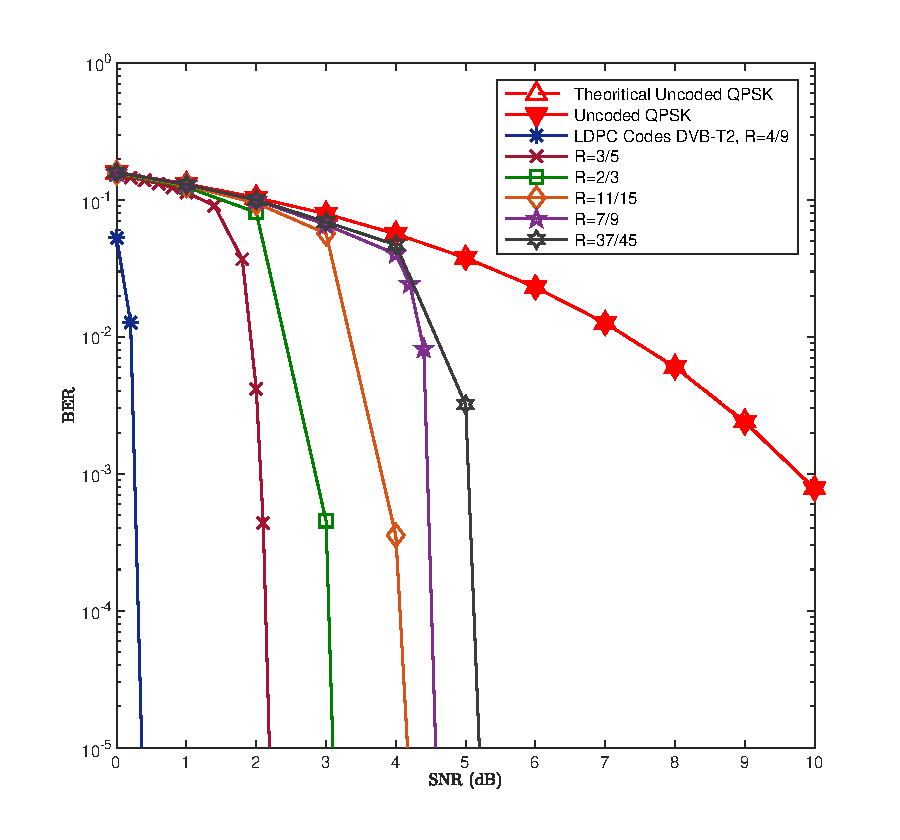
\includegraphics[width=1\textwidth]
	{hasiloriAWGN.pdf}
	\caption{Kinerja BER LDPC \textit{codes} DVB-T2 dengan $N_{LDPC}=16200$ pada kanal AWGN.}
	\label{fig:awgnori}
\end{figure}


\begin{figure}[H]
	\centering
	%	\hspace{-0.2 in}
	\begin{minipage}{1\linewidth}
		\hspace{0.75 cm}
		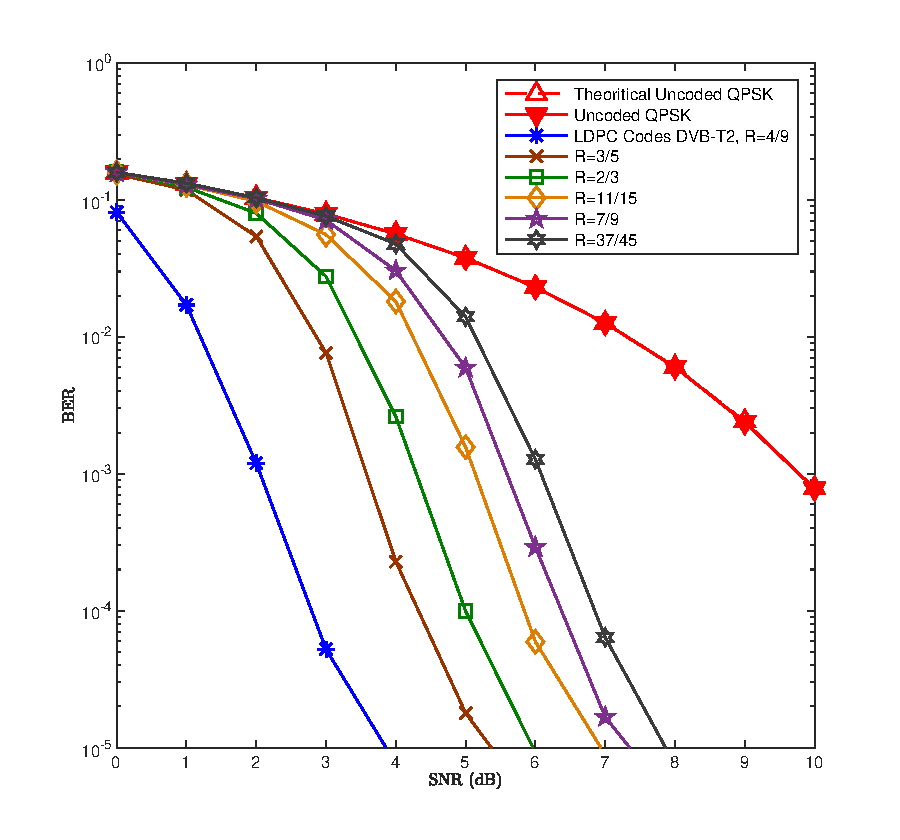
\includegraphics[width=0.85\textwidth]{hasildsfix.pdf}
		\vspace{-1cm}
		
		\center  (a)
	\end{minipage}
	\hfill
	\begin{minipage}{1\linewidth}
		\hspace{0.75 cm}
		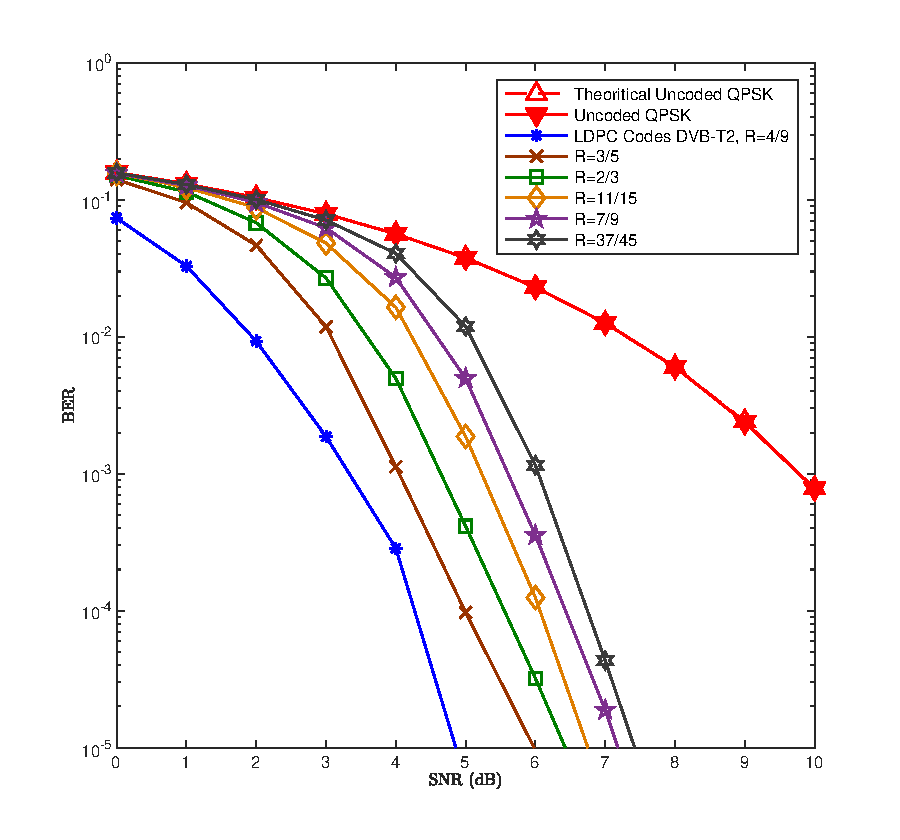
\includegraphics[width=0.85\textwidth]{hasilpegawgnfix.pdf}
		\vspace{-1cm}
		\center (b)
	\end{minipage}
	%	\begin{minipage}{.5\linewidth}
	%		\hspace{-0.4 cm}
	%		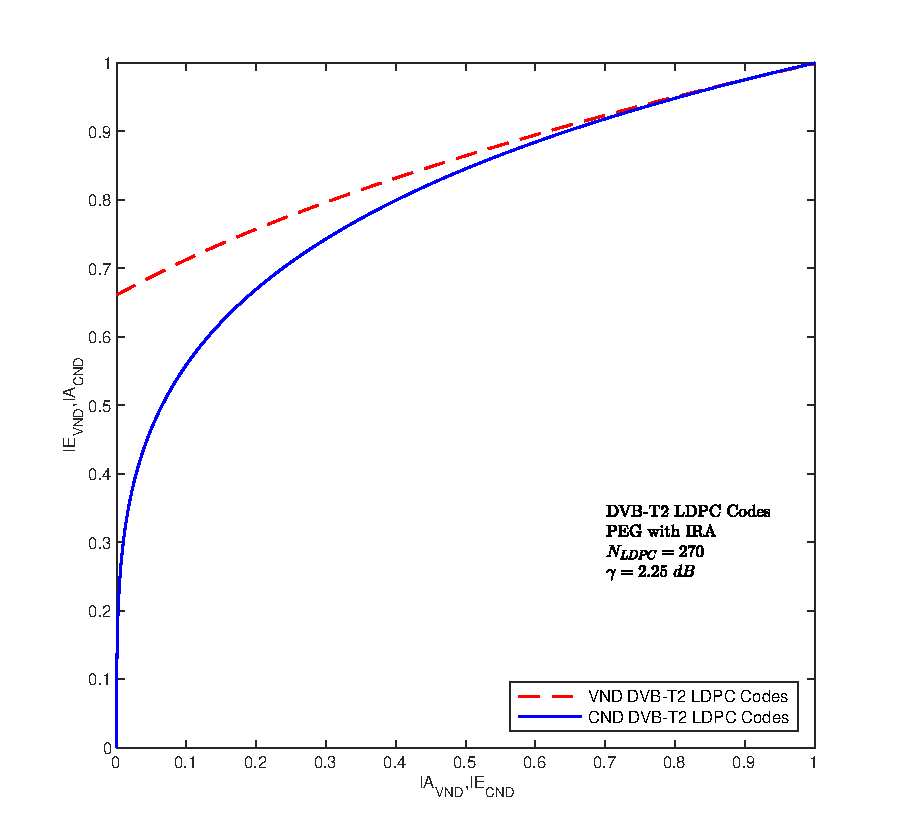
\includegraphics[width=3in]{pics/exit/12/12peg=snr2,25Ich=0,6613.pdf}
	%		\vspace{-1cm}
	%		\center (c)
	%	\end{minipage}
	\caption {Kinerja BER LDPC \textit{codes} DVB-T2 dengan: (a) $N_{LDPC}=270$ menggunakan metode \textit{downscaling} dan (b) $N_{LDPC}=270$ menggunakan PEG dengan \textit{accumulator} pada kanal AWGN.}
	\label{gambar:dspeg}
\end{figure}

Gambar \ref{fig:awgnori} menunjukkan perbandingan kinerja original LDPC \textit{codes} DVB-T2 untuk semua \textit{code rate} pada kanal AWGN dengan teori BER QPSK dan \textit{uncoded} QPSK, LDPC \textit{codes} DVB-T2 yang diusulkan terbukti dapat memiliki kinerja BER yang jauh lebih baik daripada teori BER QPSK dan tanpa \textit{channel coding} (\textit{uncoded}) QPSK. Gambar \ref{gambar:dspeg} (a) menunjukkan perbandingan kinerja \textit{downscaled} LDPC \textit{codes} DVB-T2 untuk semua \textit{code rate} pada kanal AWGN dengan teori BER QPSK dan \textit{uncoded} QPSK, sedangkan Gambar \ref{gambar:dspeg} (b) menunjukkan perbandingan kinerja \textit{downscaled} LDPC \textit{codes} DVB-T2 yang dikombinasikan dengan \textit{accumulator} untuk semua \textit{code rate} pada kanal AWGN dengan teori BER QPSK dan \textit{uncoded} QPSK. Gambar \ref{fig:pegldgm} menunjukkan perbandingan kinerja \textit{downscaled} LDPC \textit{codes} DVB-T2 yang dikombinasikan dengan LDGM untuk semua \textit{code rate} pada kanal AWGN dengan teori BER QPSK dan \textit{uncoded} QPSK.


\begin{figure}[b!]
	\centering
	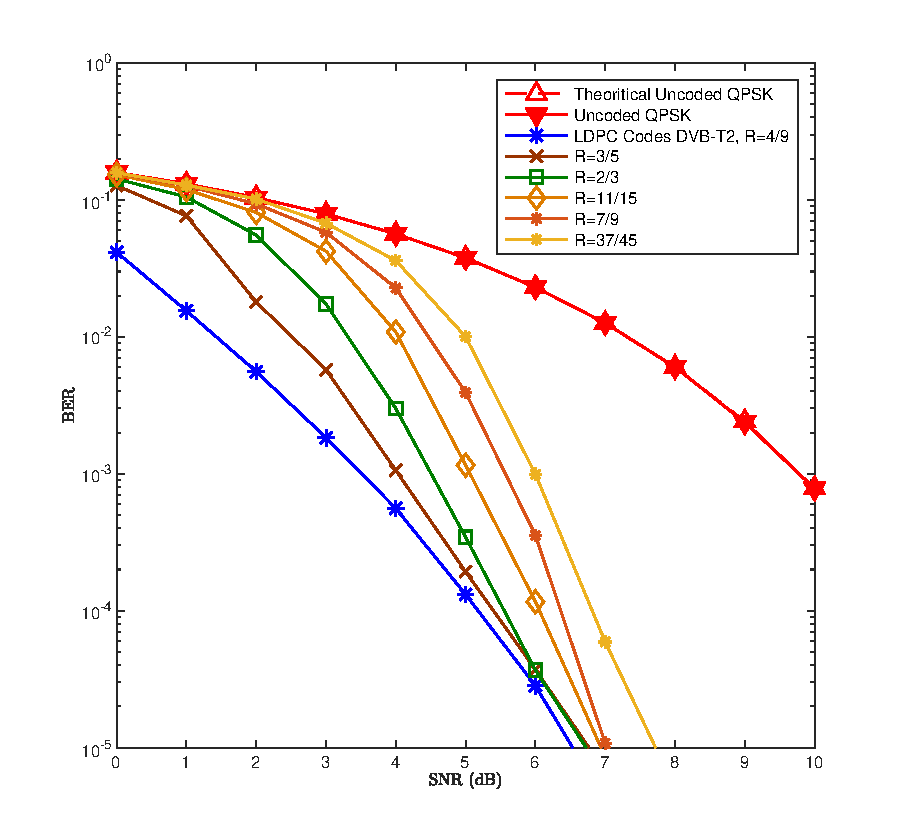
\includegraphics[width=1\textwidth]
	{hasilpegawgnfixLDGM.pdf}
	\caption{Kinerja BER LDPC \textit{codes} DVB-T2 dengan $N_{LDPC}=270$ menggunakan PEG dengan LDGM pada kanal AWGN.}
	\label{fig:pegldgm}
\end{figure}

Kinerja BER LDPC \textit{codes} DVB-T2 yang diusulkan terbukti dapat memiliki kinerja BER yang jauh lebih baik daripada teori BER QPSK dan \textit{uncoded} QPSK.
%Kinerja BER \textit{downscaled} LDPC codes dengan menggunakan PEG memiliki kinerja yang lebih baik daripada metode downscaled normal.
 Tabel \ref{tabel:hasilawgn} menunjukkan bahwa semakin besar panjang blok pada LDPC \textit{codes} yang digunakan, maka LDPC \textit{codes} akan memiliki kinerja lebih baik. Tabel \ref{tabel:hasilawgn}  menunjukkan bahwa gap kinerja antara original dan \textit{downscaled} LDPC \textit{codes} rata-rata $2~dB$ pada setiap \textit{code rate}.

\begin{table*} [t]
	\centering
	\caption{Perbandingan kinerja LDPC \textit{codes} DVB-T2 yang diusulkan pada kanal AWGN.}
	\label{tab:tab1}
%	\begin{tabular}{|c|c|c|c|}
%		\hline
%		\rowcolor[HTML]{FFCB2F} 
%		\multicolumn{1}{|c|}{\cellcolor[HTML]{FFCB2F}\textbf{Code rate}} & \textbf{Original LDPC \textit{codes}} & \textbf{\textit{Downscaled} LDPC \textit{codes}} & \textbf{PEG LDPC \textit{codes}} \\ \hline
%		$R_e=\frac{4}{9}$ & 160 & 160 & 128 \\ \hline
%		$R_e=\frac{3}{5}$ & 1 $\times$ 832 & 1 $\times$ 672 & 1 $\times$ 544 \\ \hline
%		$R_e=\frac{2}{3}$ & 160 $\times$ 832 & 160 $\times$ 672 & 128 $\times$ 544 \\ \hline
%		$R_e=\frac{11}{15}$ & 672 $\times$ 832 & 512 $\times$ 672 & 416 $\times$ 544 \\ \hline
%		$R_e=\frac{7}{9}$ & 692.224 & 451.584 & 295.936 \\ \hline
%				$R_e=\frac{37}{45}$ & 692.224 & 451.584 & 295.936 \\ \hline
%	\end{tabular}
%\begin{tabular}{|c|c|c|c|}
%	\hline
%	\multicolumn{4}{|c|}{Analisis SNR terhadap BER $= 10^{-4}$}     \\
%	\hline
%%	\rowcolor[HTML]{FFCB2F}
%	\textit{Code rate} & Original LDPC \textit{codes} & \textit{Downscaled} LDPC \textit{codes} & PEG LDPC \textit{codes} \\ \hline
%	\xrowht[()]{10pt}
%	$R_e=\frac{4}{9}$ & $0,2~dB$ & $2,83~dB$ & $3,5~dB$ \\ \hline \xrowht[()]{10pt}
%			$R_e=\frac{3}{5}$ & $2,1~dB$  & $4,1~dB$ & $4,9~dB$\\ \hline \xrowht[()]{10pt}
%			$R_e=\frac{2}{3}$ & $3,1~dB$ & $5~dB$ & $5,3~dB$ \\ \hline \xrowht[()]{10pt}
%			$R_e=\frac{11}{15}$ & $4,1~dB$ & $5,8~dB$ & $5,6~dB$ \\ \hline \xrowht[()]{10pt}
%			$R_e=\frac{7}{9}$ & $4,4~dB$ & $6,15~dB$ & $6,25~dB$ \\ \hline \xrowht[()]{10pt}
%					$R_e=\frac{37}{45}$ & $5,1~dB$ & $7~dB$ & $6,5~dB$ \\ \hline
%\end{tabular}
\begin{adjustbox}{width=1\textwidth , totalheight=\textheight-2\baselineskip,keepaspectratio}
	\begin{tabular}{|c|p{2.75cm}|p{2.75cm}|p{2.75cm}|p{2.75cm}|}
	\hline
	\multicolumn{5}{|c|}{\large \thead{ Analisis SNR terhadap $BER = 10^{-4}$}}    \\
	\hline
	%	\rowcolor[HTML]{FFCB2F}
		\thead{ \large \textit{Code rate}} & \thead{ \large Original \\LDPC} & \large \thead{ \textit{Downscaled} \\LDPC }& \large \thead{ PEG LDPC \\\textit{accumulator} } & \large \thead{ PEG LDPC \\LDGM} \xrowht[()]{0.65pt}
 \\ \hline
	\xrowht[()]{15pt}
	\large $R_e=\frac{4}{9}$ & \large $0,2~dB$ &  \large $2,83~dB$ & \large $4,25~dB$ & \large $5,15~dB$ \\ \hline \xrowht[()]{15pt}
	\large $R_e=\frac{3}{5}$ &\large $2,1~dB$  &\large $4,1~dB$ &\large $5,1~dB$ &\large $5,25~dB$ \\ \hline \xrowht[()]{15pt}
	\large $R_e=\frac{2}{3}$ &\large $3,1~dB$ &\large $5~dB$ &\large $5,5~dB$ &\large $5,35~dB$ \\ \hline \xrowht[()]{15pt}
	\large $R_e=\frac{11}{15}$ &\large $4,1~dB$ &\large $5,8~dB$ &\large $6,2~dB$ &\large $6~dB$ \\ \hline \xrowht[()]{15pt}
	\large $R_e=\frac{7}{9}$ &\large $4,4~dB$ &\large $6,15~dB$ &\large $6,4~dB$ &\large $6,25~dB$ \\ \hline \xrowht[()]{15pt}
	\large $R_e=\frac{37}{45}$ &\large $5,1~dB$ &\large $7~dB$ &\large $6.85~dB$ &\large $6,85~dB$ \\ \hline
\end{tabular}
	            \end{adjustbox}

\label{tabel:hasilawgn}
\end{table*}



%\begin{figure}
%	\centering
%%	\hspace{ -0.1in}
%	\begin{minipage}{.5\linewidth}
%		\hspace{-1.75cm}
%		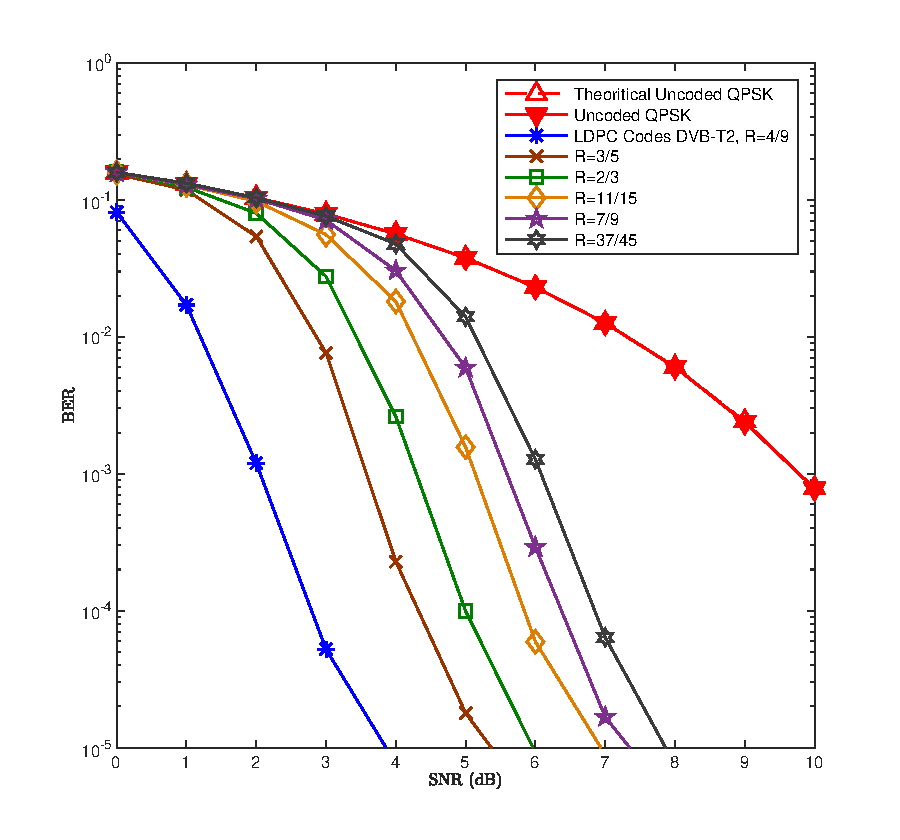
\includegraphics[width=4in]{hasildsfix.pdf}
%		\vspace{-1.5cm}
%		
%		\center (a)
%	\end{minipage}
%	\hfill 	
%%	\hspace{ -0.1in}
%	\begin{minipage}{.5\linewidth}
%		\hspace{-1.75cm}
%		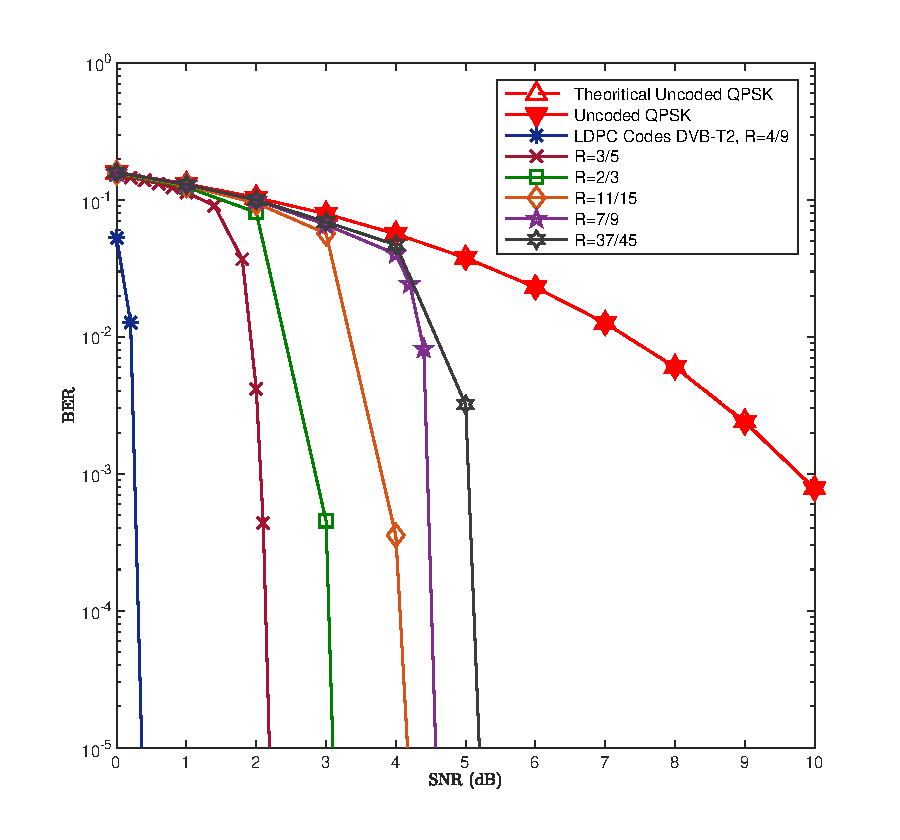
\includegraphics[width=4in]{hasiloriAWGN.pdf}
%		
%%		\vspace{-0.85cm}
%		\vspace{-0.75cm}
%
%		\center 
%%		\hspace*{0.75cm}
%		(b)
%	\end{minipage}
%	\hfill
%%	\begin{minipage}{.5\linewidth}
%%		\hspace{-1.5cm}
%%		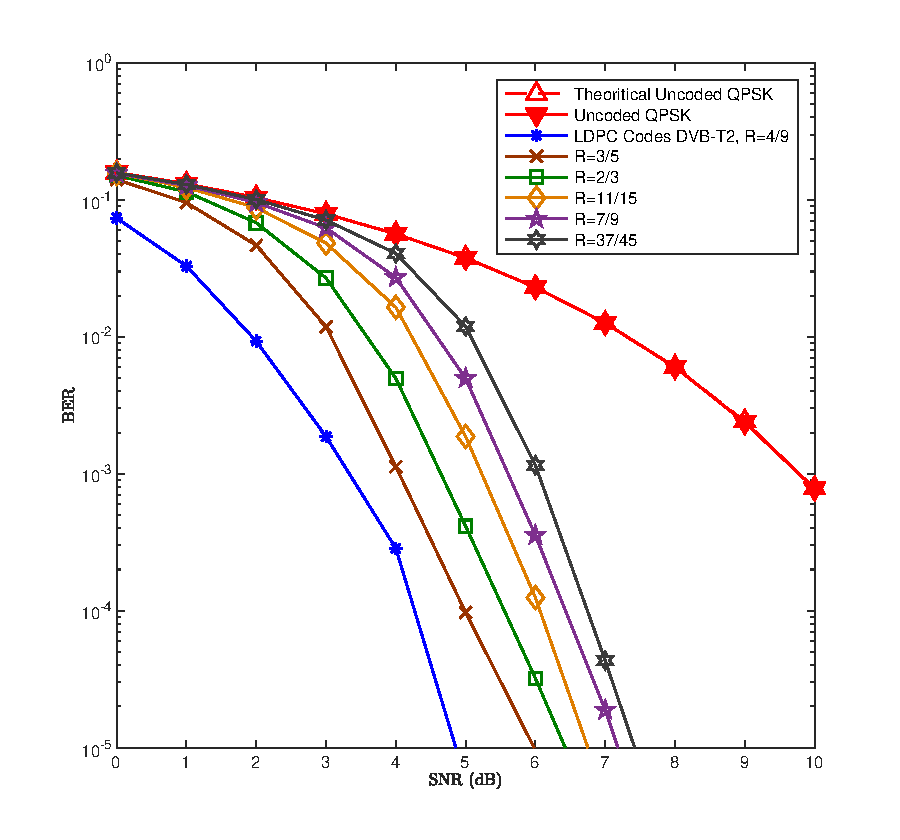
\includegraphics[width=4in]{hasilpegawgnfix.pdf}
%%		\vspace{-1.5cm}
%%		\center (c)
%%	\end{minipage}
%%	\hspace{-0.1 in}
%%	\begin{minipage}{.5\linewidth}
%%%		\hspace{2.25 cm}
%%		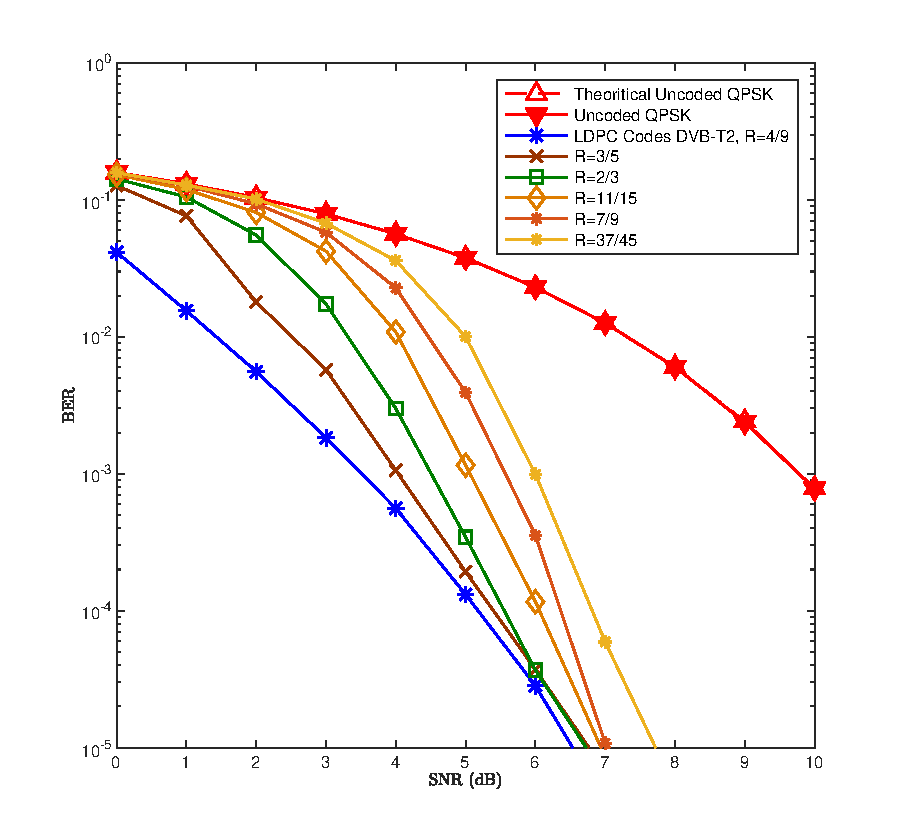
\includegraphics[width=4in]{hasilpegawgnfixLDGM.pdf}
%%		\vspace{-1.5cm}
%%		\center \hspace*{0.75cm}(d)
%%	\end{minipage}
%	\caption {Kinerja BER LDPC \textit{codes} DVB-T2 dengan: (a) $N_{LDPC}=270$ menggunakan metode \textit{downscaling} dan (b) $N_{LDPC}=16200$ kanal AWGN .}
%	\label{gambar: awgnhasil}
%\end{figure}
%
%\begin{figure}
%	\centering
%%	\hspace{ -0.1in}
%%	\begin{minipage}{.5\linewidth}
%%		\hspace{-1.75cm}
%%		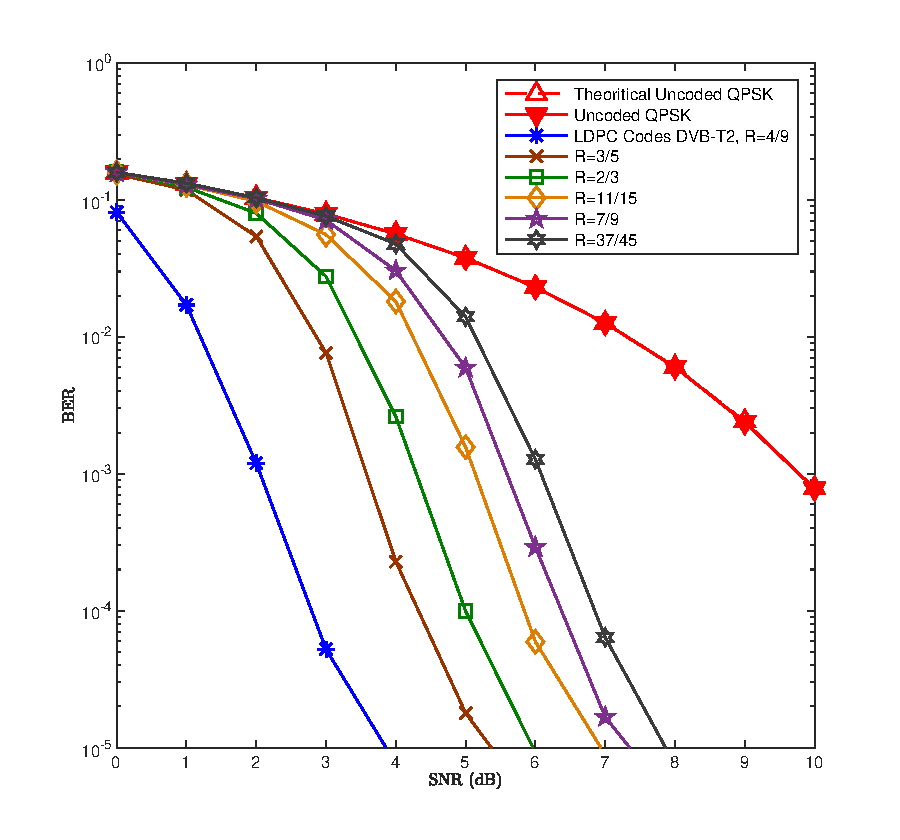
\includegraphics[width=4in]{hasildsfix.pdf}
%%		\vspace{-1.5cm}
%%		
%%		\center (a)
%%	\end{minipage}
%%	\hfill 	
%%%	\hspace{ -0.1in}
%%	\begin{minipage}{.5\linewidth}
%%		\hspace{-1.75cm}
%%		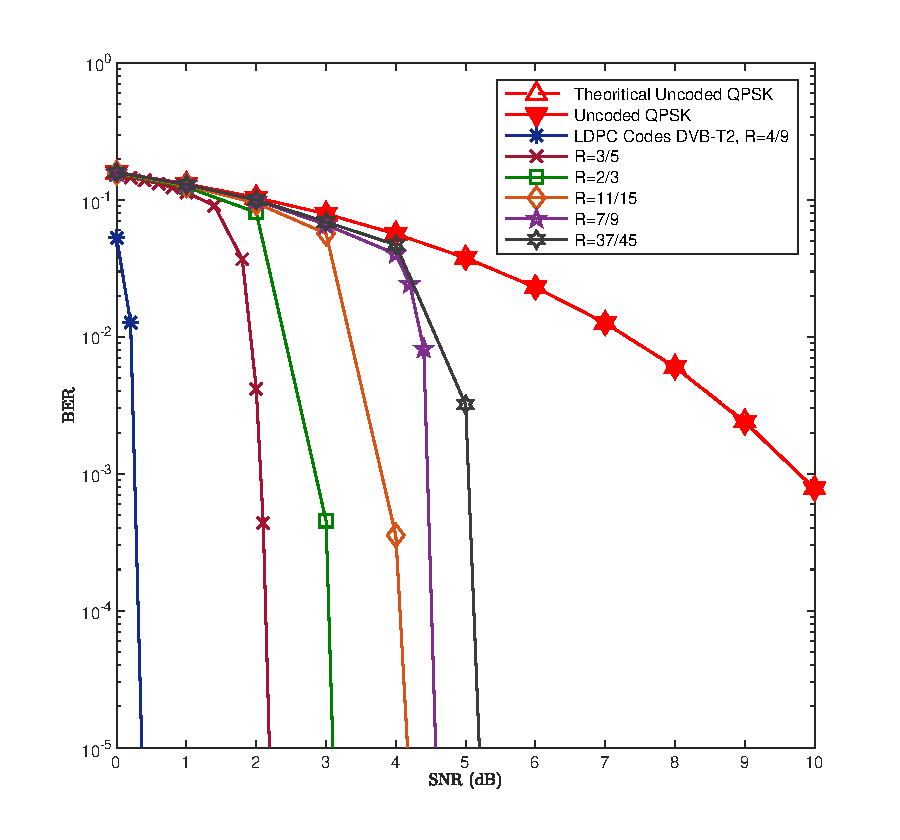
\includegraphics[width=4in]{hasiloriAWGN.pdf}
%%		
%%%		\vspace{-0.85cm}
%%		\vspace{-0.75cm}
%%
%%		\center 
%%%		\hspace*{0.75cm}
%%		(b)
%%	\end{minipage}
%%	\hfill
%	\begin{minipage}{.5\linewidth}
%	\hspace{-1.75cm}
%		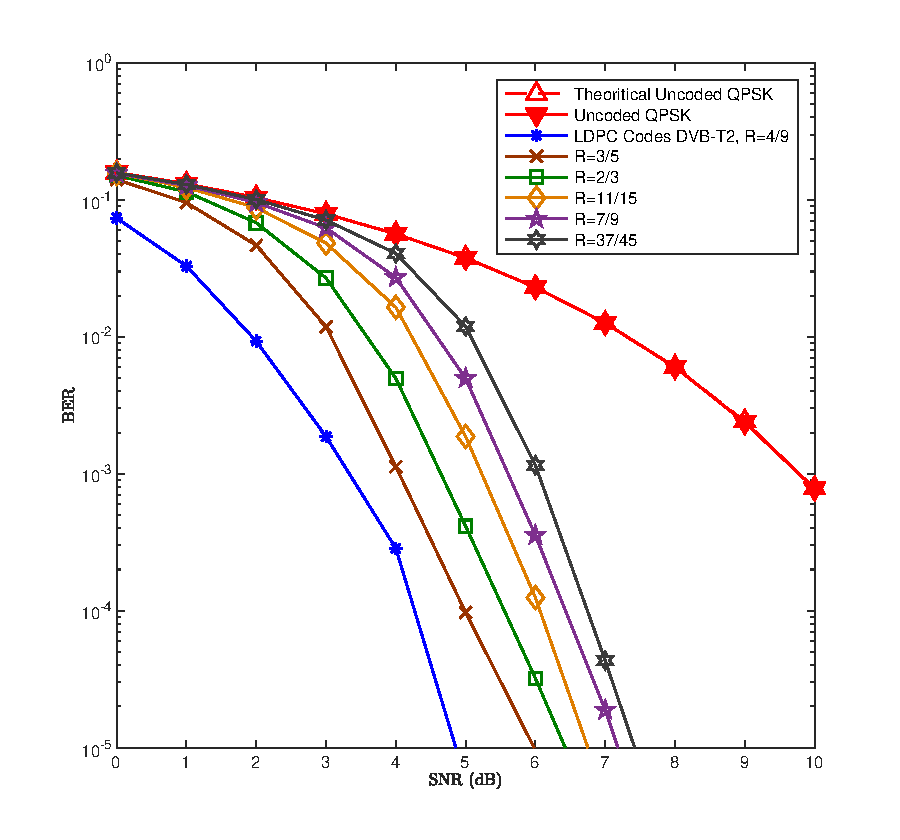
\includegraphics[width=4in]{hasilpegawgnfix.pdf}
%		\vspace{-1.5cm}
%		\center (a)
%	\end{minipage}
%%	\hspace{-0.1 in}
%	\begin{minipage}{.5\linewidth}
%		\hspace{-1.75 cm}
%		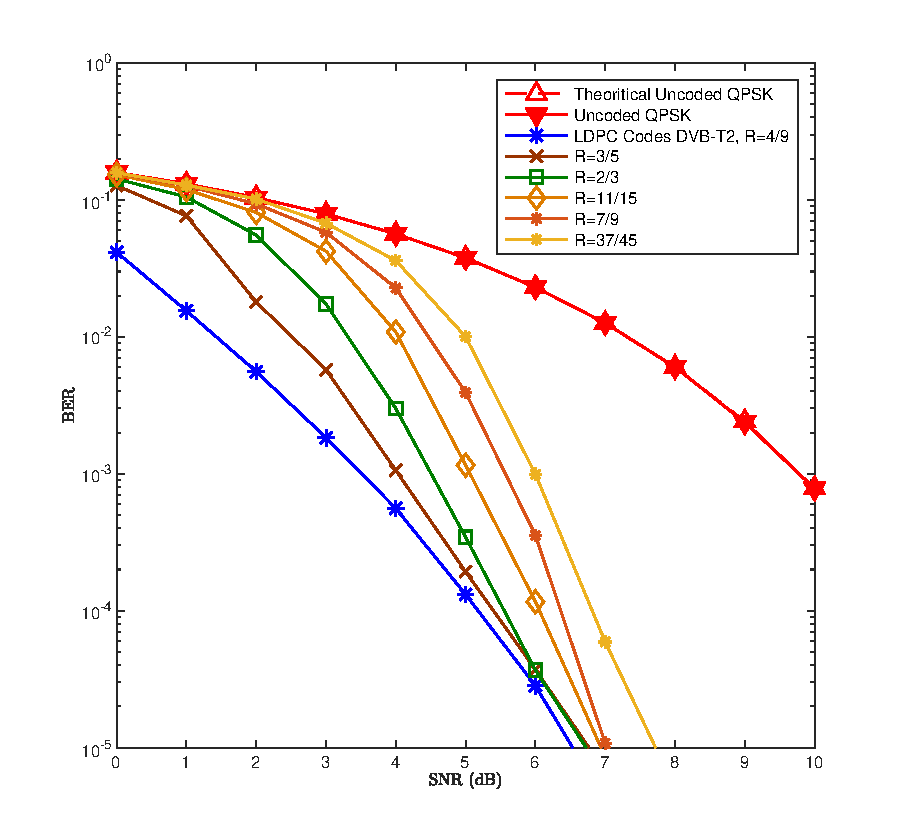
\includegraphics[width=4in]{hasilpegawgnfixLDGM.pdf}
%%		\vspace{-0.75cm}
%				\vspace{-1.5cm}
%
%		\center 
%%		\hspace*{0.75cm}
%		(b)
%	\end{minipage}
%	\caption {Kinerja BER LDPC \textit{codes} DVB-T2 dengan: (a) $N_{LDPC}=270$ menggunakan PEG dengan \textit{Accumulator} dan (b) $N_{LDPC}=270$ menggunakan PEG dengan LDGM pada kanal AWGN.}
%	\label{gambar: awgnhasilpeg}
%\end{figure}

%
%\begin{figure}
%	\centering
%	\hspace{ -0.1in}
%	\begin{minipage}{.5\linewidth}
%		\hspace{-1.15cm}
%		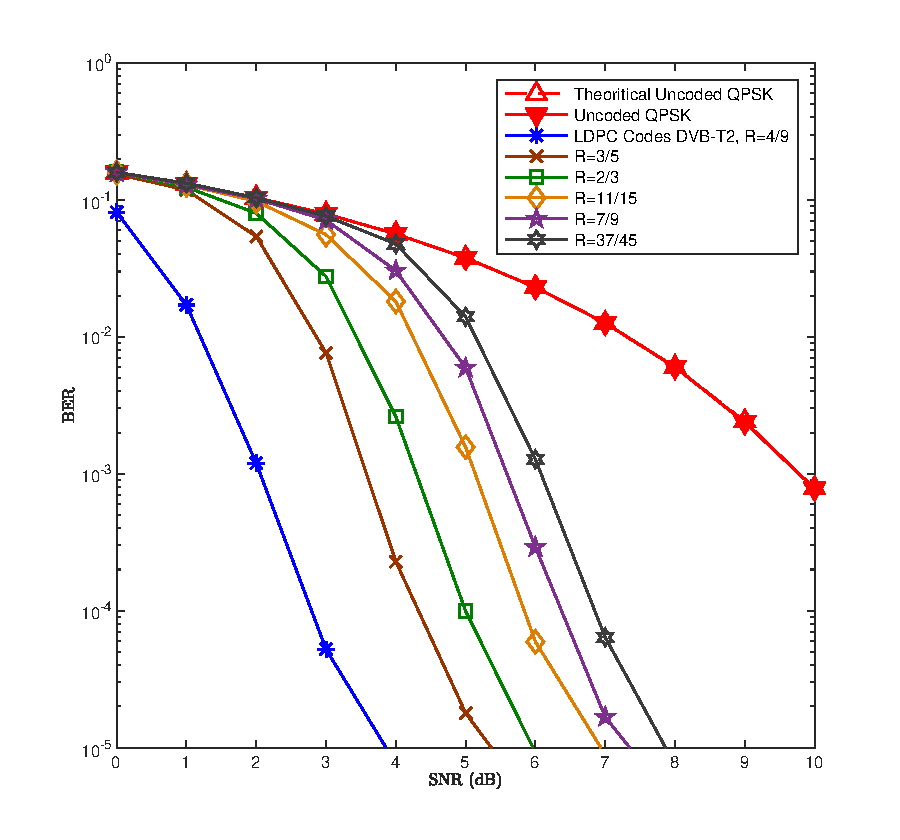
\includegraphics[width=3.5in]{hasildsfix.pdf}
%		\vspace{-1.5cm}
%		
%		\center (a)
%	\end{minipage}
%	\hfill 	\hspace{ -0.1in}
%	\begin{minipage}{.5\linewidth}
%%		\hspace{2.25 cm}
%		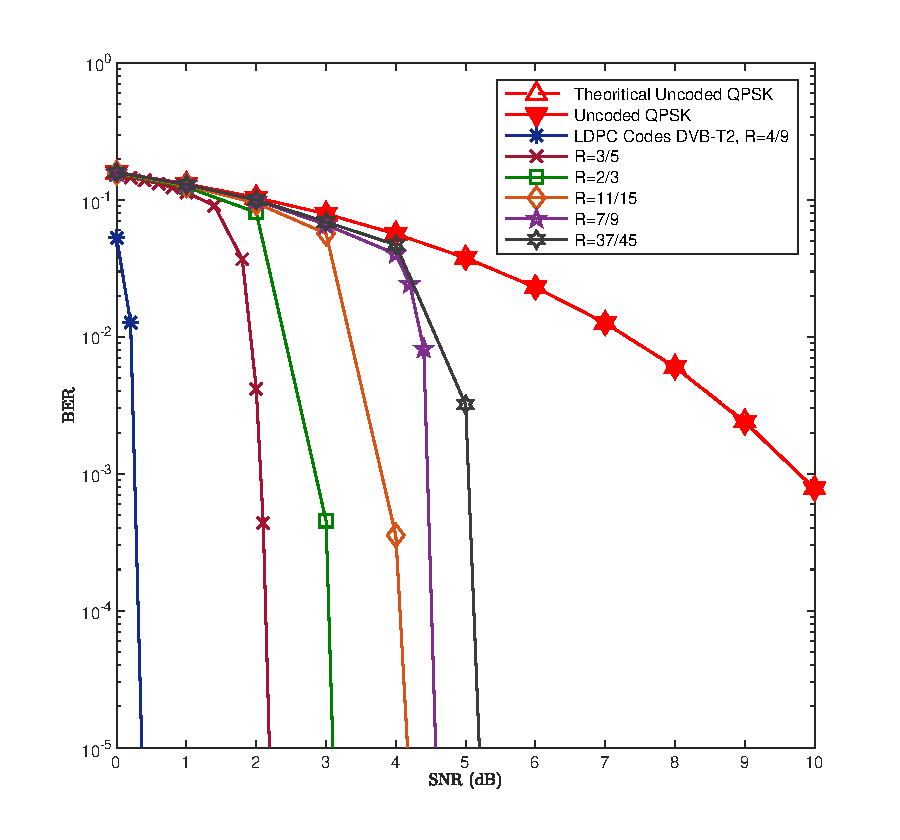
\includegraphics[width=3.5in]{hasiloriAWGN.pdf}
%		
%		\vspace{-0.95cm}
%		\center \hspace*{2.25cm}(b)
%	\end{minipage}
%	
%	\begin{minipage}{.5\linewidth}
%		\hspace{-1.25cm}
%		\includegraphics[width=3.5in]{hasilpegawgnfix.pdf}
%		\vspace{-1.5cm}
%		\center (c)
%	\end{minipage}
%	\hfill \hspace{-0.1 in}
%	\begin{minipage}{.5\linewidth}
%%		\hspace{2.25 cm}
%		\includegraphics[width=3.5in]{hasilpegawgnfixLDGM.pdf}
%		\vspace{-1.5cm}
%		\center \hspace*{2.25cm}(d)
%	\end{minipage}
%	\caption {Kinerja BER LDPC \textit{codes} DVB-T2 dengan: (a) $N_{LDPC}=270$ menggunakan metode \textit{downscaling}, (b) $N_{LDPC}=16200$, (c) $N_{LDPC}=270$ menggunakan PEG dengan \textit{accumulator}, dan (d) $N_{LDPC}=270$ menggunakan PEG dengan LDGM pada kanal AWGN.}
%	\label{gambar: awgnhasil}
%\end{figure}
%
%\clearpage


%\begin{figure}
%	\centering
%	\hspace{ -0.1in}
%	\begin{minipage}{.5\linewidth}
%		\hspace{-0.5cm}
%		\includegraphics[width=3in]{hasildsfix.pdf}
%		\vspace{-1.5cm}
%		
%		\center (a)
%	\end{minipage}
%	\hfill 	\hspace{ -0.1in}
%	\begin{minipage}{.5\linewidth}
%%		\hspace{cm}
%		\includegraphics[width=3in]{hasiloriAWGN.pdf}
%		
%		\vspace{-0.85cm}
%		\center \hspace*{0.75cm}(b)
%	\end{minipage}
%	\hfill
%	\begin{minipage}{.5\linewidth}
%		\hspace{-0.5cm}
%		\includegraphics[width=3in]{hasilpegawgnfix.pdf}
%		\vspace{-1.5cm}
%		\center (c)
%	\end{minipage}
%	\hspace{-0.1 in}
%	\begin{minipage}{.5\linewidth}
%%		\hspace{2.25 cm}
%		\includegraphics[width=3in]{hasilpegawgnfixLDGM.pdf}
%		\vspace{-1.5cm}
%		\center \hspace*{0.75cm}(d)
%	\end{minipage}
%	\caption {Kinerja BER LDPC \textit{codes} DVB-T2 dengan: (a) $N_{LDPC}=270$ menggunakan metode \textit{downscaling}, (b) $N_{LDPC}=16200$, (c) $N_{LDPC}=270$ menggunakan PEG dengan \textit{Accumulator}, dan (d) $N_{LDPC}=270$ menggunakan PEG dengan LDGM pada kanal AWGN .}
%	\label{gambar: awgnhasil}
%\end{figure}

%Tabel \ref{label} menunjukkan kinerja BER LDPC c

%\begin{figure}
%	\centering
%	\hspace{-0.2 in}
%	\begin{minipage}{.5\linewidth}
%		\hspace{-0.4 cm}
%		\includegraphics[width=3in]{hasilOFDMdsfix.pdf}
%		\vspace{-1cm}
%		
%		\center (a)
%	\end{minipage}
%	\hfill
%	\begin{minipage}{.5\linewidth}
%		\hspace{-0.4 cm}
%		\includegraphics[width=3in]{hasilOFDMpegfix.pdf}
%
%		\vspace{-1cm}
%		\center (b)
%	\end{minipage}
%\begin{minipage}{.5\linewidth}
%	\hspace{2.25 cm}
%	\includegraphics[width=3in]{hasilOFDMaslifix.pdf}
%	
%	\vspace{-0.5cm}
%	\center (b)
%\end{minipage}
%\begin{minipage}{.5\linewidth}
%	\hspace{2.25 cm}
%	\includegraphics[width=1.5in]{hasilOFDMpegfixLDGM.pdf}
%	\vspace{-0.5cm}
%	\center (d)
%\end{minipage}
%	\caption {Kinerja BER LDPC \textit{codes} DVB-T2 dengan: (a) $N_{LDPC}=270$ menggunakan PEG, (b) $N_{LDPC}=270$ menggunakan metode \textit{downscaled}, dan (c) $N_{LDPC}=16200$ pada \textit{channel model} DVB-T2 Kota Bandung.}
%	\label{gambar: ofdmhasil}
%\end{figure}





\subsection{Kinerja pada \textit{Channel Model} DVB-T2 Indonesia}
%Tugas Akhir ini mengevaluasi dan menampilkan kinerja BER LDPC \textit{codes} DVB-T2 pada \textit{channel model} DVB-T2 Kota Bandung yang diharapkan dapat menjadi referensi untuk implementasi DVB-T2 di Indonesia. 

\begin{table*} [t!]
	\centering
	\caption{Perbandingan kinerja LDPC \textit{codes} DVB-T2 yang diusulkan pada \textit{channel model} DVB-T2 Kota Bandung.}
	
	%	\begin{tabular}{|c|c|c|c|}
	%		\hline
	%		\multicolumn{4}{|c|}{Analisis SNR terhadap BER $= 10^{-4}$}     \\
	%		\hline
	%		%	\rowcolor[HTML]{FFCB2F}
	%		\textit{Code rate} & Original LDPC \textit{codes} & \textit{Downscaled} LDPC \textit{codes} & PEG LDPC \textit{codes} \\ \hline
	%		\xrowht[()]{10pt}
	%		$R_e=\frac{4}{9}$ & $0,2~dB$ & $2,83~dB$ & $3,5~dB$ \\ \hline \xrowht[()]{10pt}
	%		$R_e=\frac{3}{5}$ & $2,1~dB$  & $4,1~dB$ & $4,9~dB$\\ \hline \xrowht[()]{10pt}
	%		$R_e=\frac{2}{3}$ & $3,1~dB$ & $5~dB$ & $5,3~dB$ \\ \hline \xrowht[()]{10pt}
	%		$R_e=\frac{11}{15}$ & $4,1~dB$ & $5,8~dB$ & $5,6~dB$ \\ \hline \xrowht[()]{10pt}
	%		$R_e=\frac{7}{9}$ & $4,4~dB$ & $6,15~dB$ & $6,25~dB$ \\ \hline \xrowht[()]{10pt}
	%		$R_e=\frac{37}{45}$ & $5,1~dB$ & $7~dB$ & $6,5~dB$ \\ \hline
	%	\end{tabular}
	\begin{adjustbox}{width=1\textwidth , totalheight=\textheight-2\baselineskip,keepaspectratio}
		\begin{tabular}{|c|p{2.75cm}|p{2.75cm}|p{2.75cm}|p{2.75cm}|}
			\hline
			\multicolumn{5}{|c|}{\large \thead{Analisis SNR terhadap $BER = 10^{-4}$}}     \\
			\hline
			%	\rowcolor[HTML]{FFCB2F}
			\large	\thead{\textit{Code rate} }&\large \thead{Original \\LDPC  }&\large \thead{ \textit{Downscaled} \\LDPC} &\large \thead { PEG LDPC \\ \textit{accumulator} }&\large \thead{PEG LDPC \\ LDGM }\\ \hline
			\xrowht[()]{15pt}
			\large $R_e=\frac{4}{9}$ &\large $4~dB$ & \large $15~dB$ &\large $16~dB$ &\large $17,15~dB$ \\ \hline \xrowht[()]{15pt}
			\large $R_e=\frac{3}{5}$ &\large $9~dB$  &\large $17,5~dB$ &\large $17~dB$ &\large $18,5~dB$\\ \hline \xrowht[()]{15pt}
			\large $R_e=\frac{2}{3}$ &\large $11,1~dB$ &\large $18,5~dB$ &\large $18,5~dB$ &\large $18,95~dB$\\ \hline \xrowht[()]{15pt}
			\large $R_e=\frac{11}{15}$ &\large $14,25~dB$ &\large $22~dB$ &\large $19,4~dB$ &\large $20~dB$\\ \hline \xrowht[()]{15pt}
			\large $R_e=\frac{7}{9}$ &\large $14,95~dB$ &\large $23~dB$ &\large $22~dB$ &\large $21,15~dB$\\ \hline \xrowht[()]{15pt}
			\large $R_e=\frac{37}{45}$ & \large $17,1~dB$ &\large  $24~dB$ &\large $23,5~dB$ &\large $24,15~dB$\\ \hline
		\end{tabular}
	\end{adjustbox}
	\label{tabel:hasilOFDM}
\end{table*}

Tugas Akhir ini membandingkan hasil kinerja BER dengan teori BER pada kanal \textit{single path} (\textit{Rayleigh fading}) dan BER untuk \textit{uncoded} QPSK pada \textit{channel model} DVB-T2 Kota Bandung dalam SNR $\gamma$ yang ditunjukkan pada Tabel \ref{tabel:hasilOFDM}. 


Sistem OFDM mengharuskan setiap simbol yang dikirim pada satu blok atau \textit{frame} sama dengan jumlah FFT \textit{size}, sedangkan bit yang dikirimkan LDPC \textit{codes} untuk setiap \textit{frame}-nya pun bersifat tetap. Oleh karena itu, Tugas Akhir ini menggunakan teknik penambahan \textit{dummy} pada pengirim untuk mengisi bit yang kosong pada OFDM, kemudian pada penerima \textit{dummy} akan dilepas sebelum di-\textit{decode}, \textit{dummy} diletakkan di bagian belakang bit yang akan dikirimkan.

 \begin{figure}[tb!]
	\centering
	\includegraphics[width=1\textwidth]
	{hasilOFDMaslifix2.pdf}
	\caption{Kinerja BER LDPC \textit{codes} DVB-T2 dengan $N_{LDPC}=16200$ pada \textit{channel model} DVB-T2 Kota Bandung.}
	\label{fig:ofdmori}
\end{figure}

Khusus untuk LDPC \textit{codes} dengan $N_{LDPC}=16200$ yang ditunjukkan pada Gambar \ref{fig:ofdmori} karena keterbatasan simulasi komputer, Tugas Akhir ini menggunakan metode \textit{slicing} pada \textit{codeword} yang terbentuk. \textit{Codeword} dipotong-potong seukuran dengan FFT \textit{size} 256. Sebelum proses \textit{decoding} LLR yang terpotong-potong digabungkan kembali menjadi satu.

\begin{figure}[b!]
	\centering
	\includegraphics[width=1\textwidth]
	{hasilOFDMdsfix2.pdf}
	\caption{Kinerja BER \textit{downscaled} LDPC \textit{codes} DVB-T2 dengan $N_{LDPC}=270$ pada \textit{channel model} DVB-T2 Kota Bandung.}
	\label{fig:ofdmds}
\end{figure}

 Tugas Akhir ini menyajikan analisis daya dalam SNR terhadap kinerja pada $BER=10^{-4}$ berdasarkan modulasi QPSK pada sistem OFDM dengan FFT \textit{size} $256$ dan panjang CP sebesar $8$. Gambar \ref{fig:ofdmori} menunjukkan perbandingan kinerja original LDPC \textit{codes} DVB-T2 untuk semua \textit{code rate} pada \textit{channel model} DVB-T2 Bandung dengan teori BER \textit{singlepath} QPSK dan \textit{uncoded} QPSK. Gambar \ref{fig:ofdmds} menunjukkan perbandingan kinerja \textit{downscaled} LDPC \textit{codes} DVB-T2 untuk semua \textit{code rate} pada \textit{channel model} DVB-T2 Bandung dengan teori BER \textit{singlepath} QPSK dan \textit{uncoded} QPSK. Gambar \ref{gambar:peg} (a) menunjukkan perbandingan kinerja \textit{downscaled} LDPC \textit{codes} DVB-T2 yang menggunakan \textit{accumulator} untuk semua \textit{code rate} pada \textit{channel model} DVB-T2 Bandung, sedangkan Gambar \ref{gambar:peg} (b) menunjukkan perbandingan kinerja \textit{downscaled} LDPC \textit{codes} DVB-T2 yang menggunakan LDGM untuk semua \textit{code rate} pada \textit{channel model} DVB-T2 Bandung.

 
 \begin{figure}[H]
 	\centering
 	%	\hspace{-0.2 in}
 	\begin{minipage}{1\linewidth}
 		\hspace{0.75 cm}
 		\includegraphics[width=0.85\textwidth]{hasilOFDMpegfix2.pdf}
 		\vspace{-1cm}
 		
 		\center  (a)
 	\end{minipage}
 	\hfill
 	\begin{minipage}{1\linewidth}
 		\hspace{0.75 cm}
 		\includegraphics[width=0.85\textwidth]{hasilOFDMpegfixLDGM2.pdf}
 		\vspace{-1cm}
 		\center (b)
 	\end{minipage}
 	%	\begin{minipage}{.5\linewidth}
 	%		\hspace{-0.4 cm}
 	%		\includegraphics[width=3in]{pics/exit/12/12peg=snr2,25Ich=0,6613.pdf}
 	%		\vspace{-1cm}
 	%		\center (c)
 	%	\end{minipage}
 	\caption {Kinerja BER LDPC \textit{codes} DVB-T2 dengan: (a) $N_{LDPC}=270$ menggunakan PEG dengan \textit{accumulator}, dan (b) $N_{LDPC}=270$ menggunakan PEG dengan LDGM pada \textit{channel model} DVB-T2 Kota Bandung.}
 	\label{gambar:peg}
 \end{figure}
 
  Tabel \ref{tabel:hasilOFDM} menunjukkan LDPC \textit{codes} DVB-T2 dan sistem yang diusulkan memiliki kinerja  yang baik pada \textit{channel model} DVB-T2 di wilayah Indonesia. Kinerja BER pada \textit{channel model} DVB-T2 Bandung menunjukkan bahwa LDPC \textit{codes} DVB-T2 dengan \textit{code rate} $R_e=\frac{4}{9}$ memiliki kinerja terbaik pada \textit{channel model} DVB-T2 Bandung untuk \textit{downscaled} maupun original LDPC \textit{codes} dan menunjukkan bahwa PEG dengan \textit{accumulator} \textit{codes} memiliki kinerja yang lebih baik daripada LDGM \textit{codes}.
  

 
% \begin{figure}[H]
% 	\centering
% 	%	\hspace{-0.2 in}
% 	\begin{minipage}{1\linewidth}
% 		\hspace{0.75 cm}
% 		\includegraphics[width=0.85\textwidth]{hasildsfix.pdf}
% 		\vspace{-1cm}
% 		
% 		\center  (a)
% 	\end{minipage}
% 	\hfill
% 	\begin{minipage}{1\linewidth}
% 		\hspace{0.75 cm}
% 		\includegraphics[width=0.85\textwidth]{hasilpegawgnfix.pdf}
% 		\vspace{-1cm}
% 		\center (b)
% 	\end{minipage}
% 	%	\begin{minipage}{.5\linewidth}
% 	%		\hspace{-0.4 cm}
% 	%		\includegraphics[width=3in]{pics/exit/12/12peg=snr2,25Ich=0,6613.pdf}
% 	%		\vspace{-1cm}
% 	%		\center (c)
% 	%	\end{minipage}
% 	\caption {Kinerja BER LDPC \textit{codes} DVB-T2 dengan: (a) $N_{LDPC}=270$ menggunakan metode \textit{downscaling} dan (b) $N_{LDPC}=270$ menggunakan PEG dengan \textit{accumulator} pada kanal AWGN.}
% 	\label{gambar:dspeg}
% \end{figure}
 
 
% Gambar \ref{gambar: ofdmhasil} menunjukkan kinerja BER LDPC \textit{codes} \text{dengan} $N_{LDPC}=16200$, \textit{downscaled} LDPC \textit{codes} dengan $N_{LDPC}=270$, \textit{downscaled} menggunakan PEG LDPC \textit{codes} DVB-T2 dengan \textit{accumulator}, dan \textit{downscaled} menggunakan PEG LDPC \textit{codes} DVB-T2 dengan LDGM.
 
 
%Sistem OFDM mengharuskan setiap simbol yang dikirim pada satu blok atau \textit{frame} sama dengan jumlah FFT \textit{size}, sedangkan bit yang dikirimkan LDPC \textit{codes} untuk setiap \textit{frame}-nya pun bersifat tetap. Oleh karena itu, Tugas Akhir ini menggunakan teknik penambahan \textit{dummy} pada pengirim untuk mengisi bit yang kosong pada OFDM, kemudian pada penerima \textit{dummy} akan dilepas sebelum di-\textit{decode}, \textit{dummy} diletakkan di bagian belakang bit yang akan dikirimkan.
%
%
%Khusus untuk LDPC \textit{codes} dengan $N_{LDPC}=16200$ karena keterbatasan simulasi komputer, Tugas Akhir ini menggunakan metode \textit{slicing} pada \textit{codeword} yang terbentuk. \textit{Codeword} dipotong-potong seukuran dengan FFT \textit{size} 256. Sebelum proses \textit{decoding} LLR yang terpotong-potong digabungkan kembali menjadi satu.
%
%\begin{figure}
%	\centering
%	\hspace{ -0.1in}
%	\begin{minipage}{.5\linewidth}
%		\hspace{-1.15cm}
%		\includegraphics[width=3.5in]{hasilOFDMdsfix.pdf}
%		\vspace{-1.5cm}
%		
%		\center (a)
%	\end{minipage}
%	\hfill 	\hspace{ -0.1in}
%	\begin{minipage}{.5\linewidth}
%%		\hspace{2.25 cm}
%		\includegraphics[width=3.5in]{hasilOFDMaslifix.pdf}
%		
%		\vspace{-0.95cm}
%		\center \hspace*{2.25cm}(b)
%	\end{minipage}
%	
%	\begin{minipage}{.5\linewidth}
%		\hspace{-1.25cm}
%		\includegraphics[width=3.5in]{hasilOFDMpegfix.pdf}
%		\vspace{-1.5cm}
%		\center (c)
%	\end{minipage}
%	\hfill \hspace{-0.1 in}
%	\begin{minipage}{.5\linewidth}
%%		\hspace{2.25 cm}
%		\includegraphics[width=3.5in]{hasilOFDMpegfixLDGM.pdf}
%		\vspace{-1.5cm}
%		\center \hspace*{2.25cm}(d)
%	\end{minipage}
%	\caption {Kinerja BER LDPC \textit{codes} DVB-T2 dengan: (a) $N_{LDPC}=270$ menggunakan metode \textit{downscaled}, (b) $N_{LDPC}=16200$, (c) $N_{LDPC}=270$ menggunakan PEG dengan \textit{accumulator}, dan (d) $N_{LDPC}=270$ menggunakan PEG dengan LDGM pada \textit{channel model} DVB-T2 Kota Bandung.}
%	\label{gambar: ofdmhasil}
%\end{figure}
%\clearpage



\begin{figure}[tb]
	\centering
	\hspace{-0.25 cm}
	\begin{minipage}{.5\linewidth}
				\hspace{-0.35 cm}
		\includegraphics[width=3in]{pics/girth/girthds4-9.pdf}
		\vspace{-1cm}
			\center (a)
	\end{minipage}
\hfill
%	\hspace{-0.8 cm}
	\begin{minipage}{.5\linewidth}
		\hspace{-0.45 cm}
		\includegraphics[width=3in]{pics/girth/girthds3-5.pdf}
		\vspace{-1cm}
		\center (b)
	\end{minipage}
	\hspace{-0.2 cm}
	\begin{minipage}{.5\linewidth}
		\hspace{-0.45 cm}
		\includegraphics[width=3in]{pics/girth/girthds2-3.pdf}
		\vspace{-1cm}
		\center (c)
	\end{minipage}
\hfill
	\hspace{-0.2 cm}
\begin{minipage}{.5\linewidth}
		\hspace{-0.45 cm}
	\includegraphics[width=3in]{pics/girth/girthds3-4.pdf}
	\vspace{-1cm}
	\center (d)
\end{minipage}
	\hspace{-0.2 cm}
\begin{minipage}{.5\linewidth}
		\hspace{-0.45 cm}
	\includegraphics[width=3in]{pics/girth/girthds7-9.pdf}
	\vspace{-1cm}
	\center (e)
\end{minipage}
\hfill
	\hspace{-0.2 cm}
\begin{minipage}{.5\linewidth}
		\hspace{-0.45 cm}
	\includegraphics[width=3in]{pics/girth/girthds37-45.pdf}
	\vspace{-1cm}
	\center (f)
\end{minipage}
	\caption {Distribusi \textit{girth} \textit{downscaled} LDPC \textit{codes} DVB-T2 dengan \textit{code rate} $R_e$: (a) $ R_e=\frac{4}{9} $, (b) $R_e=\frac{3}{5}$, (c) $R_e=\frac{2}{3}$, (d) $R_e=\frac{11}{15}$, (e) $R_e=\frac{7}{9}$, dan (f) $R_e=\frac{37}{45}$.}
	\label{gambar: girthds}
\end{figure}

\section{Evaluasi \textit{Girth} LDPC \textit{Codes}}
Tugas Akhir ini mengevaluasi jumlah \textit{girth} dari setiap LDPC \textit{codes} DVB-T2 yang diusulkan. \textit{Girth} dihitung menggunakan teknik yang telah diusulkan oleh Tugas Akhir ini. Gambar \ref{gambar: girthds} dan \ref{gambar: girthpeg} menunjukkan distribusi dari \textit{girth} yang terbentuk pada \textit{downscaled} LDPC \textit{codes} DVB-T2 di setiap \textit{variable node}. Gambar \ref{gambar: girthds} menunjukkan bahwa pada \textit{downscaled} LDPC \textit{codes} DVB-T2 yang terbentuk di setiap \textit{code rate}-nya memiliki nilai \textit{girth} sebesar 4, hal ini merupakan parameter yang perlu dihindari dalam sebuah LDPC \textit{codes} karena akan memperburuk proses \textit{iterative decoding} pada LDPC \textit{codes}. Tugas Akhir ini mengusulkan \textit{downscaled} LDPC \textit{codes} yang dirancang dengan menggunakan PEG. Gambar \ref{gambar: girthpeg} menunjukkan bahwa \textit{downscaled} LDPC \textit{codes} DVB-T2 yang dirancang menggunakan PEG menghasilkan \textit{girth} 8 untuk setiap \textit{code rate}-nya. 

Evaluasi ini menunjukkan efek dari teknik \textit{downscaling} pada LDPC \textit{codes} DVB-T2 akan menimbulkan \textit{girth} 4, padahal original LDPC \textit{codes} DVB-T2 tidak memiliki \textit{girth} 4. Oleh karena itu, \textit{downscaled} DVB-T2 LDPC \textit{codes} tidak sepenuhnya memiliki karakteristik dari original LPDC \textit{codes} dalam hal \textit{girth}. Hal ini dikarenakan semakin kecil ukuran LDPC \textit{codes}, maka kemungkinan untuk meletakkan elemen 1 untuk tidak membuat \textit{girth} 4 semakin sulit. Untuk menghindari \textit{girth} 4 diperlukan sebuah algoritma yang memperhatikan penempatan elemen 1. Algoritma PEG dan \textit{Anti Girth} 4 yang diusulkan terbukti telah berhasil untuk menghindari terbentuknya \textit{girth} 4 pada LDPC \textit{codes} yang memiliki ukuran kecil. 

%\begin{figure}[tb]
%	\centering
%%	\hspace{ -0.1in}
%	\begin{minipage}{.5\linewidth}
%	\hspace{-1.75cm}
%		\includegraphics[width=4in]{hasilOFDMdsfix.pdf}
%		\vspace{-0.75cm}
%		
%		\center (a)
%	\end{minipage}
%%	\hfill 	
%%	\hspace{ -0.1in}
%%	\hfill 	
%
%%	\hspace{ -0.1in}
%
%	\begin{minipage}{.5\linewidth}
%%		\hspace{2.25 cm}
%	\hspace{-1.75cm}
%
%		\includegraphics[width=4in]{hasilOFDMaslifix.pdf}
%		
%%		\vspace{-0.75cm}
%		\center 
%%		\hspace*{0.75cm}
%		(b)
%	\end{minipage}
%	
%%	\begin{minipage}{.5\linewidth}
%%		\hspace{-0.5cm}
%%		\includegraphics[width=3in]{hasilOFDMpegfix.pdf}
%%		\vspace{-1.5cm}
%%		\center (c)
%%	\end{minipage}
%%	\hfill \hspace{-0.1 in}
%%	\begin{minipage}{.5\linewidth}
%%%		\hspace{2.25 cm}
%%		\includegraphics[width=3in]{hasilOFDMpegfixLDGM.pdf}
%%		\vspace{-1.5cm}
%%		\center \hspace*{0.75cm}(d)
%%	\end{minipage}
%	\caption {Kinerja BER LDPC \textit{codes} DVB-T2 dengan: (a) $N_{LDPC}=270$ menggunakan metode \textit{downscaled}, (b) $N_{LDPC}=16200$, (c) $N_{LDPC}=270$ menggunakan PEG dengan \textit{accumulator}, dan (d) $N_{LDPC}=270$ menggunakan PEG dengan LDGM pada \textit{channel model} DVB-T2 Kota Bandung.}
%	\label{gambar: ofdmhasil}
%\end{figure}





%\section{Analisis LDPC \textit{codes} DVB-T2 pada Model Kanal DVB-T2 Bandung}
%
%\section{Analisis \textit{Downscaled} LDPC \textit{Codes} pada Kanal AWGN} 
%
%
%\subsection{\textit{Downscaled} Menggunakan Metode Pertama}
%
%
%\subsection{\textit{Downscaled} Menggunakan PEG}
%
%\section{Analisis \textit{Downscaled} LDPC \textit{Codes} pada Model Kanal DVB-T2 Bandung} 
%
%
%\subsection{\textit{Downscaled} Menggunakan Metode Pertama}
%
%
%\subsection{\textit{Downscaled} Menggunakan PEG}



\begin{figure}[tb]
	\centering
	\hspace{-0.25 cm}
	\begin{minipage}{.5\linewidth}
		\hspace{-0.45 cm}
		\includegraphics[width=3in]{pics/girth/girthpeg4-9.pdf}
		\vspace{-1cm}
		\center (a)
	\end{minipage}
	\hfill
	%	\hspace{-0.8 cm}
	\begin{minipage}{.5\linewidth}
		\hspace{-0.45 cm}
		\includegraphics[width=3in]{pics/girth/girthpeg3-5.pdf}
		\vspace{-1cm}
		\center (b)
	\end{minipage}
	\hspace{-0.2 cm}
	\begin{minipage}{.5\linewidth}
		\hspace{-0.45 cm}
		\includegraphics[width=3in]{pics/girth/girthpeg2-3.pdf}
		\vspace{-1cm}
		\center (c)
	\end{minipage}
	\hfill
	\hspace{-0.2 cm}
	\begin{minipage}{.5\linewidth}
		\hspace{-0.45 cm}
		\includegraphics[width=3in]{pics/girth/girthpeg11-15.pdf}
		\vspace{-1cm}
		\center (d)
	\end{minipage}
	\hspace{-0.2 cm}
	\begin{minipage}{.5\linewidth}
		\hspace{-0.45 cm}
		\includegraphics[width=3in]{pics/girth/girthpeg7-9.pdf}
		\vspace{-1cm}
		\center (e)
	\end{minipage}
	\hfill
	\hspace{-0.2 cm}
	\begin{minipage}{.5\linewidth}
		\hspace{-0.45 cm}
		\includegraphics[width=3in]{pics/girth/girthpeg37-45.pdf}
		\vspace{-1cm}
		\center (f)
	\end{minipage}
	\caption {Distribusi \textit{girth} pada \textit{downscaled} LDPC \textit{codes} DVB-T2 menggunakan PEG dengan \textit{code rate} $R_e$: (a) $ R=\frac{4}{9} $, (b) $R_e=\frac{3}{5}$, (c) $R_e=\frac{2}{3}$, (d) $R_e=\frac{11}{15}$, (e) $R_e=\frac{7}{9}$, dan (f) $R_e=\frac{37}{45}$.}
	\label{gambar: girthpeg}
\end{figure}

